\documentclass[a4paper]{article}
%Tutti gli usepackage vanno qui

\usepackage{geometry}
\usepackage[italian]{babel}
\usepackage[utf8]{inputenc}
\usepackage[T1]{fontenc}
\usepackage{tabularx}
\usepackage{longtable}
\usepackage{hyperref}
\usepackage{enumitem}
\hypersetup{
	colorlinks=true,
	linkcolor=black,
	filecolor=magenta,
	urlcolor=blue,
}
% % Numerazione figure
% \let\counterwithout\relax
% \let\counterwithin\relax
\usepackage{chngcntr}

\counterwithin{table}{subsection}
\counterwithin{figure}{subsection}

\usepackage[bottom]{footmisc}
\usepackage{fancyhdr, pageslts}
\usepackage{titlesec}
\setcounter{secnumdepth}{4}
\usepackage{amsmath, amssymb}
\usepackage{array}
\usepackage{graphicx}

%header e footer
\pagestyle{fancy}
\lhead{
\includegraphics[scale=0.11]{./res/img/logo.png}}
\rhead{Analisi dei requisiti}
\rfoot{Pagina \thepage \space di \pageref{LastPage}}
\lfoot{\small{\texttt{tenners.unipd@gmail.com}}}
\cfoot{}
\setlength{\headheight}{40pt}
\renewcommand{\footrulewidth}{0.4pt}    %linea footer fondo pagina


%tabelle
\usepackage[table]{xcolor}
\usepackage{multirow}
\definecolor{pari}{HTML}{EAEAEA}
\definecolor{dispari}{HTML}{FFFFFF}
\definecolor{header}{HTML}{b4b4b4}


%glossario
\newcommand{\glo}{$_{G}$ }
\newcommand{\glos}{$_{G}$} % pedice glossario senza spazio dopo la parola

%documento
\newcommand{\doc}{$_{D}$ }
\newcommand{\docs}{$_{D}$}

%label custom
\makeatletter
\newcommand{\uclabel}[2]{%
	\protected@write \@auxout {}{\string \newlabel {#1}{{#2}{\thepage}{#2}{#1}{}} }%
	\hypertarget{#1}{#2}
}
\makeatother

%codice
\definecolor{codegray}{gray}{0.9}
\newcommand{\code}[1]{\colorbox{codegray}{\texttt{#1}}}

\usepackage{array}
\newcolumntype{C}[1]{>{\centering\arraybackslash}p{#1}}

\pagenumbering{arabic}

\makeindex

\begin{document}
    \begin{titlepage}
	\begin{center}
		\large \textbf{Tenners - Capitolato C2}
		\vfill
		
\includegraphics[scale = 0.3]{./res/img/logo.png}\\
		\vfill
		\Huge \textbf{Verbale Interno} \\
		\textbf {2019-12-20}

        \vfill
        \large

        \begin{tabular}{r|l}
                        \textbf{Versione} & 1.0.0 \\
                        \textbf{Redazione} & Nicola Salvadore \\
                        \textbf{Verifica} &  Gianmarco Pettinato \\
                        \textbf{Approvazione} & Simone Franconetti \\
                        \textbf{Stato} & Approvato \\
                        \textbf{Uso} &  Interno\\
                        \textbf{Data creazione} &  2019-12-20\\
                        \textbf{Data ultima modifica} &  2019-12-20\\
                        \textbf{Destinatari} & \parbox[t]{5cm}{Tenners \\ Prof. Tullio Vardanega\\ Prof. Riccardo Cardin}
                \end{tabular}
                \vfill
                \normalsize
                \vfill
                \textbf{Contatto}

                \texttt{tenners.unipd@gmail.com}

	\end{center}
\end{titlepage}

    \section*{Registro delle modifiche}
\hyphenation{Incalza}
\hyphenation{Cikaqi}
\hyphenation{Trevisan}
\hyphenation{Salvadore}
\hyphenation{Ciulei}
\hyphenation{Franconetti}
\hyphenation{Pettinato}
\renewcommand{\arraystretch}{1.8}
  \rowcolors{2}{pari}{dispari}
  \setlength\LTleft{-1.7cm}
  \begin{longtable}{|p{1.7cm}|p{2cm}|p{2.5cm}|p{3cm}|p{1.7cm}|p{2cm}|p{2.3cm}|}
    \hline
    \rowcolor{header}
    \textbf{Versione} & \textbf{Nominativo} & \centering{\textbf{Ruolo}} & \textbf{Descrizione} &      \centering{\textbf{Data}} & \textbf{Verificatore} & \textbf{Data Verifica} \\
    
    3.0.0 & Giovanni Incalza & Responsabile & \small{\textit{Allineamento di versione con quella del prodotto}} & 2020-04-13 & &\\
    
    3.0.0 & Gabriel Ciulei & Verificatore & \small{\textit{Date le modifiche non retrocompatibili, si ritiene necessario uno scatto di versione}} & 2020-03-23 & &\\
    2.10.0& Simone Franconetti & Analista & \small{\textit{Aggiunto UC22}} & 2020-03-28 & Gabriel Ciulei & 2020-03-23\\
    2.9.0& Simone Franconetti & Analista & \small{\textit{Aggiunto UC14.2.1 e UC15.2.1}} & 2020-03-28 & Gabriel Ciulei & 2020-03-23\\
    2.8.1& Paola Trevisan & Analista & \small{\textit{Corretta la numerazione dei casi d'uso}} & 2020-03-22 & Gabriel Ciulei & 2020-03-23\\
    2.8.0& Paola Trevisan & Analista & \small{\textit{Eliminato UC3}} & 2020-03-22 & Gabriel Ciulei & 2020-03-23\\
    2.7.0& Nicola Salvadore & Analista & \small{\textit{Aggiunto layer in UC13 e UC14}} & 2020-03-21 & Gabriel Ciulei & 2020-03-22\\
    2.6.1& Nicola Salvadore & Analista & \small{\textit{Aggiornato UC19 - Rimozione funzione}} & 2020-03-21 & Gabriel Ciulei & 2020-03-22\\
    2.6.0& Nicola Salvadore & Analista & \small{\textit{Eliminato UC18}} & 2020-03-21 & Gabriel Ciulei & 2020-03-22\\
    2.5.0& Paola Trevisan& Analista & \small{\textit{Spostato R1Q1 in requisiti di vincolo}} & 2020-03-21 & Gabriel Ciulei & 2020-03-22\\
    2.4.2 & Gianmarco Pettinato & Responsabile & \small{\textit{Approvato per il rilascio}} & 2020-03-08 & &\\
    2.4.2-TBA & Simone Franconetti & Analista & \small{\textit{Inserite immagini per ciasuna visione a livello generale dei casi d'uso}} & 2020-03-06 & Giovanni Incalza & 2020-03-07 \\
    2.4.1-TBA & Simone Franconetti & Analista & \small{\textit{Modifica requisiti funzionali e tabelle di tracciamento}} & 2020-03-06 & Giovanni Incalza & 2020-03-07 \\
    2.4.0-TBA & Simone Franconetti & Analista & \small{\textit{Inserimento di nuovi casi d'uso (UC8.2, UC8.2.X, UC14.X, UC14.2.X, UC13.2, UC13.2.X, UC4.X)}} & 2020-03-06 & Giovanni Incalza & 2020-03-06 \\
    2.3.1-TBA & Nicola Salvadore & Analista & \small{\textit{Corretti UC9 UC8 UC5 UC19 UC18 UC16 UC15 UC14}} & 2020-02-22 & Giovanni Incalza & 2020-02-25 \\
    2.3.0-TBA & Nicola Salvadore & Analista & \small{\textit{Aggiunta gerarchia attori primari}} & 2020-02-22 & Giovanni Incalza & 2020-02-25 \\
    2.2.0-TBA & Gezim Cikaqi & Analista & \small{\textit{Aggiunti UC13.1 e UC13.2}} & 2020-02-17 & Giovanni Incalza & 2020-02-18 \\
    2.1.1-TBA & Nicola Salvadore & Analista & \small{\textit{Corretto UC16 e UC18}} & 2020-02-17 & Giovanni Incalza & 2020-02-18 \\
    2.0.0-TBA & Gezim Cikaqi & Analista & \small{\textit{Aggiornati codici dei requisiti e r2v6.2}} & 2020-02-14 & Giovanni Incalza & 2020-02-15 \\
    1.0.1-TBA & Gezim Cikaqi & Analista & \small{\textit{Correzione requisiti funzionali}} & 2020-02-14 & Giovanni Incalza & 2020-02-15 \\
    1.0.0 & Paola Trevisan & Responsabile & \small{\textit{Documento approvato per il rilascio}} & 2020-01-05 & & \\
    1.0.0-TBA & Giovanni Incalza & Verificatore & \small{\textit{Verificato raggiungimento requisiti per la versione 1.0.0}} & 2020-01-03 & & \\
    0.11.0-TBA & Simone Franconetti & Analista & \small{\textit{Redatto \textsection 4.3 e \textsection 4.4}} & 2019-12-30 & Giovanni Incalza & 2020-01-03 \\
    0.10.0-TBA & Simone Franconetti & Analista & \small{\textit{Redatto \textsection 4.1 e \textsection 4.2}} & 2019-12-28 & Giovanni Incalza & 2020-01-03 \\
    0.9.1-TBA & Gianmarco Pettinato & Analista & \small{\textit{Modificato \textsection 3.2.15, \textsection 3.2.20, \textsection 3.2.26 e \textsection 3.2.30}} & 2019-12-28 & Giovanni Incalza & 2020-01-03 \\
    0.9.0-TBA & Simone Franconetti & Analista & \small{\textit{Redatto \textsection 3.2.39 - \textsection 3.2.41}} & 2019-12-26 & Gezim Cikaqi & 2019-12-27\\
    0.8.0-TBA & Simone Franconetti & Analista & \small{\textit{Redatto \textsection 3.2.33 - \textsection 3.2.38}} & 2019-12-24 & Gezim Cikaqi & 2019-12-24 \\
    0.7.0-TBA & Simone Franconetti & Analista & \small{\textit{Redatto \textsection 3.2.31 - \textsection 3.2.33}} & 2019-12-23 & Gezim Cikaqi & 2019-12-24 \\
    0.6.0-TBA & Simone Franconetti & Analista & \small{\textit{Redatto \textsection 3.2.23 - \textsection 3.2.30}} & 2019-12-21 & Gezim Cikaqi & 2019-12-24 \\
    0.5.0-TBA & Simone Franconetti & Analista & \small{\textit{Redatto \textsection 3.2.15 - \textsection 3.2.22}} & 2019-12-20 & Giovanni Incalza & 2019-12-18 \\
    0.4.0-TBA & Simone Franconetti & Analista & \small{\textit{Redatto \textsection 3.2.8 - \textsection 3.2.15}} & 2019-12-19 & Giovanni Incalza & 2019-12-18 \\
    0.3.0-TBA & Simone Franconetti & Analista & \small{\textit{Redatto \textsection 3.1 e \textsection 3.2.1 - \textsection 3.2.7}} & 2019-12-17 & Nicola Salvadore & 2019-12-18\\
    0.2.1-TBA & Gabriel Ciulei & Analista & \small{\textit{Modifica \textsection 2.2 e \textsection 2.3}} & 2019-12-15 & Giovanni Incalza & 2019-12-16 \\
    0.2.0-TBA & Gabriel Ciulei & Analista & \small{\textit{Redatto \textsection 2.3 e \textsection 2.4}} & 2019-12-14 & Giovanni Incalza & 2019-12-16 \\
    0.1.0-TBA & Gabriel Ciulei & Analista & \small{\textit{Redatto \textsection 1, \textsection 2.1 e \textsection 2.2}} & 2019-12-13 & Giovanni Incalza & 2019-12-16\\
    0.0.1-TBA & Gabriel Ciulei & Analista & \small{\textit{Creata la struttura del documento}} & 2019-12-13 & Giovanni Incalza & 2019-12-16 \\
    \hline
  \end{longtable}
\setlength\LTleft{0cm}

    \tableofcontents
    \newpage
    \listoffigures
    \newpage
    %\listoftables
    \section{Introduzione}

\subsection{Scopo del Documento}
Questo documento si prefigge di dichiarare le strategie atte a garantire la qualit\'a \glo, definendo quindi i processi di verifica \glo e validazione \glo. Saranno presentate qui non solo le politiche trasversali all'intera organizzazione Tenners, ma anche gli obiettivi da perseguire sul progetto intero. Sar\'a necessario quindi rendere note le procedure e gli strumenti di controllo attraverso le quali ci prefissiamo di raggiungere la qualit'a \glo.
\'E necessario specificare che il documento non \'e statico, ma cambier\'a durante tutta la durata del progetto. Infatti, molte delle politiche o dei processi selezionati inizialmente potranno rivelarsi insufficienti o inadeguati, costringendoci a modificare o aggiungerli. Il piano di qualifica \glo sar\'a prodotto in maniera incrementale e i cambiamenti saranno tracciati nella sezione del registro delle modifiche.

\subsection{Scopo del prodotto}
Il capitolato C2 ha come obbiettivo una piattaforma per svilippatori che metta
in comunicazione un fornitore di funzionalit\`a e chi \`e interessato ad utilizzarle
all'interno del proprio progetto.
La piattaforma prender\`a nome di etherless permettendo a chi sviluppa software e
lo condivide sulla piattaforma di essere pagato, per ogni esecuzione, attraverso
la criptovaluta etherium.


\subsection{Glossario}
Come supporto alla documentazione, viene fornito un \textit{Glossario v.1.0.0},
contenente le definizioni di termini specifici che necessitano di un chiarimento.
Ognuno di questi verr\`a contrassegnato con un pedice \glo nel documento e la sua
spiegazione verr\`a riportata sotto la corrispondente lettera del glossario. Ci\`o
consentir\`a di avere un linguaggio comune ed evitare ambiguit\`a.

\subsection{Rifermenti}
\subsubsection{Rifermenti normativi}
\begin{enumerate}
  \item Piano di qualifica in particola la sezione legata al capitolato C6.
\end{enumerate}
\subsubsection{Rifermenti informativi}
\begin{enumerate}
  \item ISO Standards
	\url{https://www.praxiom.com/}
\end{enumerate}


    \section{Processi Primari}
\subsection{Processi di Fornitura}
\subsubsection{Scopo}
Lo scopo del processo di Fornitura è quello di delineare le risorse e le procedure da utilizzare nello svolgimento del progetto. Si propone, quindi di normare tutti i comportamenti che il gruppo Tenners deve tenere con i proponenti e i committenti al fine di diventare quindi fornitori degli stessi.
\subsubsection{Aspettative}
I componenti del gruppo sperano di intrattenere una comunicazione stretta con i proponenti, in modo tale da assodare subito eventuali dubbi e avere consigli su come effettivamente procedere.
\subsubsection{Attività}
\paragraph{Studio di Fattibilità}
Lo Studio di Fattibilità si prefigge di raccogliere le impressioni del gruppo relativi ai capitolati presentati. Il documento è stato redatto cercando di raggiungere un compromesso su tutte le opinioni dei componenti di Tenners. Per ogni capitolato viene indicato:
\begin{itemize}
  \item \textbf{Descrizione Generale}: viene esposto in sintesi il contenuto del capitolato, indicando nome del progetto e il proponente.
  \item \textbf{Finalità del Progetto}: viene presentato il capitolato più in dettaglio specificando lo scopo del Progetto.
  \item \textbf{Tecnologie Interessate}:vengono elencate le possibili tecnologie interessate nel progetto.
  \item \textbf{Aspetti positivi}: viene spiegato perché secondo il gruppo sia favorevole scegliere questo capitolato.
  \item \textbf{Criticità}: vengono esposte le eventuali problematiche nello sviluppo di un progetto su questo capitolato.
  \item \textbf{Valutazione Conclusiva}: viene riportata la discussione del gruppo e le conclusioni a cui è giunto.
\end{itemize}
\paragraph{Piano di Progetto}
Quali attività svolgere e dove allocare le risorse è indicato nel Piano del progetto. I responsabili e gli amministratori del progetto si occuperanno di distribuirle nel periodo del progetto, in modo da rendere il Piano di Progetto il più efficiente possibile. Questo documento deve contenere le seguenti sezioni:
\begin{itemize}
  \item \textbf{Analisi dei Rischi}: vengono individuati i possibili rischi e errori che possono palesarsi durante il progetto. Inoltre, vengono esposti eventuali soluzioni o azioni preventive per evitarli.
  \item \textbf{Modello di Sviluppo}: definizione del ciclo di vita scelto e utilizzato per il progetto.
  \item \textbf{Pianificazione}: vengono definite le scadenze temporali per ciascuna attività e i ruoli ai quali assegnare le stesse.
  \item \textbf{Preventivo e Consuntivo}: viene stimato il tempo necessario a ciascuna attività e di conseguenza i presunto costo totale del progetto. Viene anche stilato un documento detto Consuntivo, per quanto riguarda l'andamento dello sviluppo del progetto e la differenza con ciò che é stato preventivato.
\end{itemize}
\paragraph{Piano di Qualifica}
Lo scopo del piano di Qualifica è quello di definire le tecniche di verifica e validazione. In particolare chi è stato assegnato a questo compito, i verificatori, saranno tenuti a garantire:
\begin{itemize}
  \item \textbf{Qualità di Prodotto}:
\end{itemize}

    \subsection{Sviluppo}
\subsubsection{Obiettivi}
Il processo di Sviluppo coinvolge tutte le attività volte alla produzione del prodotto finale: analisi dei requisiti,  progettazione, codifica, integrazione, testing e installazione. In particolar modo, questo processo viene istanziato con i seguenti obiettivi:
\begin{itemize}
	\item definizione dei vincoli e dei requisiti del sistema finale in accordo con i bisogni espressi dagli \textit{stakeholders\glo} in causa;
	\item scomposizione e classificazione dei requisiti coinvolti;
	\item studio e analisi delle tecnologie coinvolte durante la realizzazione del sistema;
	\item realizzazione di una progettazione (architetturale e di dettaglio) basata sull'utilizzo di \textit{design pattern\glo} consolidati;
	\item implementazione del prodotto che soddisfi i requisiti esposti dal proponente e dal committente e le convenzioni stabilite all'interno del team.
\end{itemize}
\subsubsection{Attività}
\paragraph{Analisi dei requisiti}
L'analisi dei requisiti comprende la descrizione dettagliata delle specifiche del sistema. È compito dell'analista descrivere, oltre che i requisiti funzionali del prodotto, anche quelli prestazionali, di qualità e di vincolo.
Questa attività ha come obiettivo il perseguimento delle seguenti caratteristiche:
\begin{itemize}
	\item \textbf{Chiarezza strutturale:} i requisiti devono essere classificati e organizzati in maniera precisa, distinguendo i requisiti funzionali da quelli non funzionali;
	\item \textbf{Chiarezza espressiva:} è necessario avere una chiarezza espositiva tale da permettere la definizione di requisiti non ambigui;
	\item \textbf{Atomicità dei requisiti:} occorre analizzare i bisogni fino a ché non si raggiungono requisiti atomici, non ulteriormente suddivisibili.
\end{itemize}

\subparagraph*{Requisiti}
L'approccio utilizzato per la definizione dei requisiti è stato di tipo \textbf{top-down}: il prodotto finale, a partire dalla sua totalità, è stato scomposto nelle parti che lo compongono sino ad arrivare a requisiti atomici. Le proprietà fondamentali di un requisito sono le seguenti:
\begin{itemize}
	\item devono essere verificabili;
	\item devono soddisfare tutti i bisogni espressi dall'utente;
	\item non devono soddisfare caratteristiche superflue (solo quelle strettamente necessarie);
	\item non devono essere contraddittori;
	\item devono essere tracciabili e modificabili.
\end{itemize}
\noindent Ogni requisito necessità tracciabilità. Verrà dunque utilizzato per ciascuno un codice identificativo strutturato nel seguente modo:
\\\\
\centerline{\textbf{[Priorità][Tipologia][Codice]}}\\
\begin{itemize}
  \item \textbf{Priorità}:
  \begin{itemize}
    \item \textbf{1 (Obbligatorio)}: necessario per almeno uno degli \textit{stakeholder\glos};
    \item \textbf{2 (Desiderabile)}: non strettamente necessario, ma di valore aggiunto;
    \item \textbf{3 (Opzionale)}: relativamente utili e contrattabili con l'avanzare del progetto.
  \end{itemize}
  \item \textbf{Tipologia}:
  \begin{itemize}
    \item \textbf{F:} funzionali;
    \item \textbf{P:} prestazionali;
    \item \textbf{Q:} qualitativi;
    \item \textbf{V:} di vincolo.
  \end{itemize}
  \item \textbf{Codice identificativo}.
\end{itemize}
Ogni requisito è opportunamente seguito da:
\begin{itemize}
  \item \textbf{Descrizione}: breve descrizione riguardante il requisito;
  \item \textbf{Fonte}: da dove proviene il requisito, chi l'ha richiesto o dove è stato ricavato. Le fonti di un requisito potranno essere le seguenti:
  \begin{itemize}
  	\item \textbf{Capitolato\glos:} se riportato nel \textit{capitolato\glos};
  	\item \textbf{Interna:} se concordato all'interno del team;
  	\item \textbf{Caso d'uso:} se derivato da un caso d'uso (verrà riportato il codice identificativo del caso d'uso come descritto nella sezione \textsection2.2.2.2);
  	\item \textbf{Verbale:} se concordato durante una riunione, verrà riportato il codice identificativo della decisione alla quale viene fatto riferimento.
  \end{itemize}
\end{itemize}

\subparagraph*{Casi d'uso}
I casi d'uso descrivono l'insieme delle casistiche con cui il sistema si interfaccia verso l'esterno. Ogni caso d'uso sarà identificato univocamente da un codice formato da:
\\\\
\centerline{\textbf{UC[Codicepadre].[Codicefiglio]}}\\

\begin{itemize}
	\item \textbf{Codicepadre:} identificativo numerico dato al caso d'uso a cui questo è associato;
	\item \textbf{Codicefiglio:} identificativo numerico per il sotto-caso corrente.
\end{itemize}
Ogni caso d'uso, oltre ad avere un relativo diagramma, verrà descritto
\begin{itemize}
  \item codice;
  \item nome;
  \item diagramma del caso d'uso;
  \item attori principali;
  \item attori secondari (opzionale);
  \item pre-condizioni;
  \item post-condizioni;
  \item scenario principale;
  \item inclusioni (opzionale);
  \item esclusioni (opzionale);
  \item specializzazioni (opzionale).
\end{itemize}

\subparagraph*{UML\glo}
Il gruppo Tenners utilizzerà la versione del linguaggio \textit{UML\glo} 2.0 per la realizzazione dei diagrammi dei casi d'uso.
\paragraph{Progettazione}
La progettazione è un'attività che si attiva al termine dell'analisi dei requisiti, ponendo le basi per l'implementazione effettiva del prodotto software. Lo scopo dei progettisti è capire come risolvere il problema di partenza e soddisfare i requisiti in modo ottimale. Diversamente da ciò che accade nell'analisi dei requisiti, in cui il problema viene progressivamente decomposto in parti più piccole, in questa attività si ricompone il tutto per definire la soluzione migliore. Si possono catalogare due tipologie di progettazione:
\begin{itemize}
	\item \textbf{progettazione architetturale:} progettazione di alto livello che descrive come il sistema deve essere organizzato nelle sue componenti;
	\item \textbf{progettazione di dettaglio:} descrive il comportamento delle singole componenti (e delle unità che le compongono) e il modo di interagire tra esse.
\end{itemize}
Nel contesto del progetto didattico, sono state stabilite due \textit{milestone}\glo distinte:
\begin{itemize}
	\item \textbf{Technology Baseline\glos}: Selezione delle tecnologie, \textit{framework}\glo e librerie tramite \textit{Proof of Concept (PoC)\glos}. Il \textit{PoC\glo} deve essere accessibile su \textit{GitHub\glos};
	\item \textbf{Product Baseline)\glos}: viene presentata una \textit{baseline\glo} architetturale coerente con quanto mostrato in Technology \textit{Baseline\glos}.
\end{itemize}
\subparagraph*{Technology Baseline\glo}
Ha lo scopo di:
\begin{itemize}
	\item motivare l'utilizzo di determinate tecnologie, \textit{framework\glo} e librerie;
	\item presentare un \textit{PoC\glo} eseguibile che venga utilizzato come \textit{baseline\glo} per l'attività di sviluppo;
	\item il codice del \textit{PoC\glo} non sarà usa e getta ma diverrà utile e necessario per i successivi incrementi del modello di sviluppo.
\end{itemize}
\subparagraph*{Product Baseline\glo}
Ha lo scopo di:
\begin{itemize}
	\item presentare la \textit{baseline\glo} architetturale del prodotto;
	\item illustrare tramite un allegato tecnico i diagrammi delle classi, di sequenza e i design pattern utilizzati contestualizzati all'architettura.
\end{itemize}
\subparagraph*{Architettura}
Il gruppo ha deciso di garantire una buona architettura perseguendo i seguenti obiettivi qualitativi:
\begin{itemize}
	\item \textbf{sufficienza:} deve soddisfare tutti i requisiti rilevati nella precedente attività di analisi;
	\item \textbf{comprensibilità:} deve poter essere compresa da tutti gli \textit{stakeholders\glo} coinvolti;
	\item \textbf{modularità:} suddivisione in parti non sovrapponibili tra loro e ben distinte;
	\item \textbf{robustezza:} gestione di un'ampia tipologia di input. Qualità strettamente legata alla modularità dell'architettura;
	\item \textbf{flessibilità:} capacità dell'architettura di evolversi e cambiare, a costi contenuti, al variare dei requisiti;
	\item \textbf{efficienza:} spreca il meno possibile in termini di spazio, tempo;
	\item \textbf{affidabilità:} esegue quello che ci si aspetta nella maniera corretta;
	\item \textbf{disponibilità:} in caso di manutenzione, il sistema rimarrà indisponibile senza aver un impatto importante sull'utenza;
	\item \textbf{sicurezza:} l'architettura non deve essere vulnerabile a intrusioni e, in caso di eventuali malfunzionamenti, deve essere garantito il funzionamento delle restanti parti dell'architettura;
	\item \textbf{semplicità:} deve soddisfare i soli requisiti necessari, eliminando funzionalità superflue;
	\item \textbf{incapsulamento:} necessità di nascondere lo stato interno esponendo solo ciò che è necessario sapere;
	\item \textbf{coesione:} presenza di coesione funzionale, sequenziale e informativa tra le componenti che costituiscono i moduli dell'architettura;
	\item \textbf{basso accoppiamento:} le componenti dell'architettura devono dipendere il meno possibile l'una dall'altra.
\end{itemize}

\subparagraph*{Diagrammi di sequenza} Descrivono uno scenario composto da una sequenza di azioni le cui scelte sono già state effettuate. Non ammette dunque flussi alternativi. Il diagramma si sviluppa su linee verticali parallele che rappresentano l'avanzare del tempo. Esso è costituito da:
\begin{itemize}
	\item \textbf{partecipanti:} entità che comunicano tra di loro;
	\item \textbf{messaggi:} dati e operazioni che vengono scambiati tra i partecipanti. Essi possono essere di diverse tipologie:
	\begin{itemize}
		\item sincroni;
		\item asincroni;
		\item di ritorno;
		\item creazione;
		\item distruzione
	\begin{figure}[h!]
		\caption{Tipologie di messaggi in un diagramma di sequenza}
		\centering
		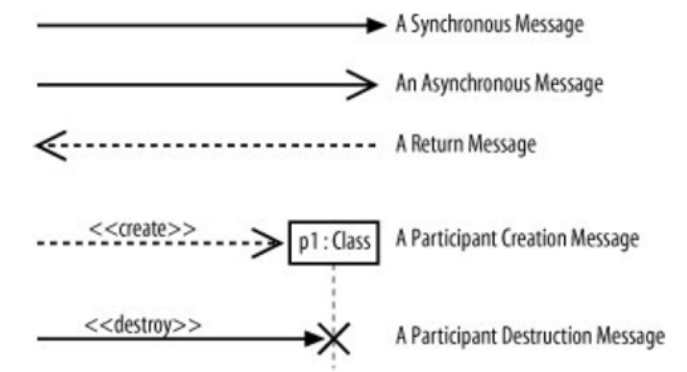
\includegraphics[width=\textwidth]{res/img/diagrammiDiSequenza.png}
	\end{figure}
	\end{itemize}
	\item \textbf{barra di attivazione:} rettangolo, posizionato sulla linea della vita di un partecipante, che ne indica il periodo di attività.
\end{itemize}

\subparagraph*{Diagrammi delle classi} Descrivono il tipo di oggetti che fanno parte di un sistema e le relazioni che intercorrono tra loro. La descrizione delle classi dovrà essere così strutturata:
\begin{itemize}
	\item \textbf{nome della classe (obbligatorio)}
	\item \textbf{attributi (feature):} Rappresentano i membri della classe. Saranno descritti nel seguente modo: \\\\ \centerline{\textbf {visibilità nome : tipo [molteplicità] = default [proprietà aggiuntive]}}\\
	\begin{itemize}
		\item visibilità:
		\begin{itemize}
			\item (+) public;
			\item (\#) protected;
			\item (~) package;
			\item (-) private.
		\end{itemize}
	\end{itemize}
	\item \textbf{operazioni (feature):} Servizi che possono essere richiesti quando si istanzierà un oggetto della classe. Saranno descritti nel seguente modo: \\\\ \centerline{\textbf {visibilità nome (lista-parametri) : tipo-ritorno [proprietà aggiuntive]}}\\\\
	dove:
	\\\\ \centerline{\textbf {lista-parametri := direzione nome : tipo = default}}\\
	\begin{itemize}
		\item visibilità:
		\begin{itemize}
			\item (+) public;
			\item (\#) protected;
			\item (~) package;
			\item (-) private.
		\end{itemize}
		\item direzione:
		\begin{itemize}
			\item in;
			\item out;
			\item in-out;
		\end{itemize}
	\end{itemize}
\end{itemize}
\noindent Tra le classi possono sussistere delle relazioni può o meno costrittive. Per raffigurarne il grado di dipendenza, vengono utilizzate le seguenti tipologie di frecce:
\begin{figure}[h!]
	\caption{Raffigurazione delle relazioni tra classi}
	\centering
	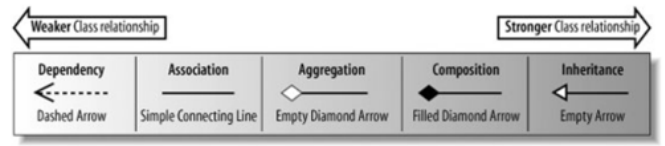
\includegraphics[width=0.8\textwidth]{res/img/relazioniClassi.png}
\end{figure}
\begin{itemize}
	\item \textbf{dipendenza:} indica una relazione breve tra gli oggetti di una classe con quelli di un'altra. Questa tipologia di relazione si verifica in due situazioni:
	\begin{itemize}
		\item un metodo di una classe "A" riceve come parametro una istanza di un'altra classe "B";
		\item la classe "A" crea un oggetto di tipo "B" in uno dei suoi metodi.
	\end{itemize}
	\item \textbf{associazione:} quando un oggetto di una classe lavora con oggetti di altre classi per un periodo prolungato. Tale relazione si verifica ad esempio nel caso in cui un attributo di una classe "A" e di tipo "B". Sarà necessario dunque, ad ogni costruzione di un oggetto di "A", costruire anche l'oggetto di tipo "B";
	\item \textbf{aggregazione:}  quando una classe possiede ma condivide un riferimento ad oggetti di
	un’altra classe. Indica, in altre parole, una relazione di tipo "parte di..";
	\item \textbf{composizione:} quando una classe "A" contiene oggetti di un’altra classe "B". In questo caso gli oggetti di tipo "B" non possono esistere senza il contenitore (tipo "A");
	\item \textbf{ereditarietà:} quando si instaurano relazioni di sottotipaggio.
\end{itemize}

\subparagraph*{Diagrammi di oggetti} Descrivono il sistema mediante gli oggetti e le associazioni tra loro. Seguono il modello descritto dai diagrammi delle classi, senza però avere alcun elemento obbligatorio. Tramite questi diagrammi è possibile inoltre verificare i valori delle proprietà associate ad un oggetto.

\subparagraph*{Diagrammi dei package} Documentano la dipendenza tra classi. Essi avranno le seguenti caratteristiche:
\begin{itemize}
	\item ogni package è caratterizzato da una etichetta che ne specifica il nome;
	\item ogni classe all'interno di un package è caratterizzata dalla visibilità che possiede nei confronti degli altri package (pubblica o privata);
\end{itemize}

\subparagraph*{Diagrammi di attività} Descrivono la logica procedurale che compone un processo. Essi sono composti da:
\begin{itemize}
	\item \textbf{nodo iniziale:} punto da cui inizia il processo;
	\item \textbf{nodo finale:} punto in cui termina il processo;
	\item \textbf{fork:} elaborazione parallela di più processi;
	\item \textbf{join:} sincronizzazione rispetto ad una determinata condizione di processi che sino a quel momento eseguivano in parallelo;
	\item \textbf{branch:} rami decisionali in cui si può intraprendere uno solo dei percorsi a disposizione.
\end{itemize}


%\subparagraph*{Diagrammi per la Progettazione}
%Per facilitare la descrizione dell'architettura del prodotto finale, si ricorre all'utilizzo di alcune tipologie di diagrammi \textit{UML\glos}:
%\begin{itemize}
%	\item \textbf{Diagrammi di sequenza:} descrivono uno scenario composto da una sequenza di azioni le cui scelte sono già state effettuate. Non ammette dunque flussi alternativi;
%	\item \textbf{Diagrammi delle classi:} descrivono il tipo di oggetti che fanno parte di un sistema;
%	\item \textbf{Diagrammi dei package:} documentano la dipendenza tra classi;
%	\item \textbf{Diagrammi di attività:} descrivono la logica procedurale che compone un processo;
%	\item \textbf{Diagrammi di oggetti:} descrivono il sistema mediante gli oggetti e le associazioni tra loro.
%\end{itemize}
\paragraph{Codifica}
Durante la Codifica viene sviluppato il codice del prodotto software dai programmatori. È fondamentale che questo risulti uniforme per migliorarne le attività di manutenzione, verifica e validazione. È quindi necessario normare il lavoro in modo tale che il loro codice risulti leggibile, attraverso uno stile di codifica.
\subparagraph*{Stile di codifica}
Stabilire convenzioni di codifica comuni, migliora la leggibilità del codice e lo rende più facilmente mantenibile. Il gruppo Tenners, per aumentare l'omogeneità e l'uniformità durante la stesura del codice richiesta da \textit{capitolato\glos}, ha scelto delle regole comuni da seguire derivanti dallo stile di codifica dettato da eslint-airbnb:
\begin{itemize}
  \item \textbf{Indentazione}: per l'indentazione dei blocchi saranno utilizzati 2 caratteri spazio (e non il classico tab), per uniformare la codifica dei caratteri su diversi sistemi operativi;
  \item \textbf{Posizione delle parentesi}: le parentesi per l'apertura di un blocco vanno inserite in linea con i costrutti mentre, quelle di chiusura, vanno inserite alla linea successiva rispetto all'ultima istruzione del blocco.
  Esempio:
  \begin{lstlisting}
  	function toCelsius(fahrenheit) {
  		return (5 / 9) * (fahrenheit - 32);
  	}
  \end{lstlisting}
  \item \textbf{Nomenclatura}: i nomi contenuti nel codice devono aderire alle seguenti convenzioni:
  \begin{itemize}
  	\item \textbf{Nome delle classi:} scritti in UpperCamelCase, senza l'utilizzo degli spazi, con la prima lettera di ciascuna parola in maiuscolo Esempio:
  	\begin{lstlisting}
  	class AccountingDepartment {
  		....
  	}
  	\end{lstlisting}
  	\item \textbf{Nome dei metodi e delle variabili:} scritti in lowerCamelCase, senza l'utilizzo degli spazi, con la prima lettera di ciascuna parola in maiuscolo eccetto la prima. Il loro nome di deve suggerire l'azione eseguita. Esempio:
  	\begin{lstlisting}
  	let z = 100;
  	function addToZ(x, y) {
  		return x + y + z;
  	}
  	\end{lstlisting}
  \end{itemize}
  Per facilitare la lettura e la comprensione del codice, tutti i nomi devono essere significativi e parlanti;
  \item \textbf{Lingua}: il codice e i commenti vanno scritti in lingua inglese;
  \item \textbf{Spazi intorno agli operatori:} verranno inseriti degli spazi intorno agli operatori ( = + - * / ) , e dopo le virgole.
  Esempio:
  \begin{lstlisting}
  var x = y + z;
  var values = [ 'Volvo', 'Saab', 'Fiat' ];
  \end{lstlisting}

\end{itemize}
%\subparagraph{TypeScript}

\subsubsection{Strumenti}
\paragraph{Visual Paradigm 13 CE}
Software utilizzato per la stesura dei diagrammi dei casi d'uso, delle classi e dei package. Permette una gestione semplice degli elementi del diagramma tramite semplici drag and drop e la versione Community Edition è disponibile gratuitamente e dunque accessibile a tutti i membri del gruppo.

\paragraph{AWS Lambda}
Servizio che consente di eseguire codice nel \textit{cloud}\glos. Esso viene utilizzato per la componente \textit{etherless-server}.

\paragraph{Visual Studio Code}
Visual Studio Code è un editor di codice sorgente che supporta, tra gli altri, il linguaggio Typescript. Tale software viene imposto dal \textit{capitolato\glos}.

\paragraph{Ethereum\glo}
Rete globale per il trasferimento di \textit{criptovalute}\glo e per la realizzazione di applicativi decentralizzati.

\paragraph{Truffle}
Framework per lo sviluppo di \textit{smart contract\glo} su rete \textit{Ethereum\glo}s.

\paragraph{Smart contract\glo}
Protocollo informatico che facilita, verifica, fa rispettare ed esegue un
contratto (insieme di regole).

\paragraph{Ropsten}
Rete \textit{Ethereum}\glo pubblica usato per il testing di applicativi \textit{Ethereum\glo} prima
del \textit{porting\glo} in produzione sulla \textit{MainNet\glos}.

\newpage \subsubsection{Linguaggi}
\paragraph{Typescript 3.6}
Versione standardizzata da Microsoft del linguaggio JavaScript.

\paragraph{Node.js}
Ambiente di runtime \textit{open-source}\glo per JavaScript.

\paragraph{Serverless\glo Framework\glo}
Framework\glo per la costruzione di ambienti serverless\glos e, in particolare, per la creazione di applicazioni su AWS Lambda.

\paragraph{Solidity}
Linguaggio OOPG per la definizione di \textit{smart contract}\glos.

\paragraph{Web3}
\textit{API}\glo JavaScript per l’interazione con un nodo \textit{Ethereum\glos}, locale o remoto.\\

\subsubsection{Procedure}
\paragraph{Visual Paradigm - Salvataggio diagramma dei casi d'uso}
\begin{enumerate}
	\item Cliccare sulla finestra "Project";
	\item Cliccare sul bottone "Export;
	\item Cliccare su "XML...";
	\item Selezionare tutti i diagrammi utilizzati tramite le checkbox;
	\item Selezionare il percorso di destinazione;
	\item Cliccare su "Export".
\end{enumerate}

\paragraph{Visual Paradigm - Caricamento diagramma dei casi d'uso}
\begin{enumerate}
	\item Cliccare sulla finestra "Project";
	\item Cliccare sul bottone "Import;
	\item Cliccare su "XML...";
	\item Digitare il percorso del file con estensione .XML;
	\item Cliccare su "Import".
\end{enumerate}


    \section{Processi di supporto}
\subsection{Documentazione}

\subsubsection{Scopo}
Questa sezione si occupa di illustrare i processi necessari alla stesura di un
documento; poiché ogni processo e attivit\`a di sviluppo significativa necessita
di documentazione, in particolare si occupa di descrivere il processo di stesura e
di gestione di testi validi.
I documenti prodotti verranno rilasciati nel repository\glo.
\href{https://github.com/Jatus93/sweDocs}{link temporaneo}

\subsubsection{Aspettative}
Le aspettative sono la definizione di norme con le quali
si gestiscono i documenti dalla creazione all'approvazione.

\subsubsection{Descrizione}
Questa parte del documento contiene le regole che sono state definite per una
migliore gestione dei documenti a cui tutti si devono attenere per produrre un
documento valido e ufficiale, senza eccezioni.

\subsubsection{Ciclo di vita del documento}
Ogni documento ha diversi stadi nel suo ciclo di vita:
\begin{itemize}
  \item \textbf{Preparazione alla creazione di un documento}: come da norme di
  sviluppo interne, per ogni nuova componente del progetto \`e necessario creare un
  feature branch\glo con il nome del componente in camel case\glo dopodich\'e
  si potr\`a creare il documento;

  \item \textbf{Creazione del documento}: il documento deve essere creato in un
  percorso che ne rifletta la destinazione d'uso, interno o esterno, e
  all'interno di una cartella che indichi il nome del del documento in
  camel case\glo che conterr\`a, al suo interno, il file main.tex;

  \item \textbf{Preparazione al primo push\glo e push in repository\glo}: prima del primo
   push bisogna modificare il file .filesToCompile con il path\glo del documento,
   questo \`e necessario alla github action\glo per testare in maniera continuativa
   la stesura del documento e fare una verifica della validit\`a del codice
   \LaTeX \space utilizzato per scriverlo;

  \item \textbf{Realizzazione}: il documento viene scritto in maniera incrementale
  considerando le osservazioni e le necessit\`a che si evidenziano nel corso del
  progetto.

  \item \textbf{Verifica automatica in un feature branch}: una volta fatto il push
  sul repository del progetto, se i file si trovano in un branch di sviluppo
  sotto feature, verranno compilati dai tool automatici segnalando eventuali errori
  nella sintassi del linguaggio \LaTeX \space utilizzato;

  \item \textbf{Richiesta di verifica manuale}: una volta terminata la verifica
  automatica il redattore segnala ai verificatori che le modifiche richieste
  sono state eseguite facendo una pull request sul branch develop;

  \item \textbf{Seconda verifica automatica}: eseguita la pull request sul branch
  develop il sistema attiva la github action di controllo relativa.

  \item \textbf{Revisione delle modifiche}: ricevuta la pull request i verificatori
  prendono in considerazione le modifiche fatte e se ritenute adeguate, faranno a
  loro volta una pull request sul branch master.

  \item \textbf{Verifica automatica e produzione automatica del documento nel
  branch develop}: Una volta nel branch develop i tool automatici produrranno il
  documento in formato pdf pronto per essere approvato del Responsabile di progetto;

  \item \textbf{Approvazione}: il Responsabile di progetto, dopo aver ricevuto la notifica
  di pull request su master, si preoccuper\`a di leggere le modifiche apportate al documento
  ed eventualmente di approvarle accettando la pull request sul branch master;

  \item \textbf{Generazione del documento}: Dopo che il documento ha raggiunto il
  branch master il sistema automatico si preoccuper\`a di creare la release del
  documento con i relativi changelog.
\end{itemize}

\subsubsection{Template}
\`E stato creato un template, che velocizza il processo di stesura verifica e
approvazione dei documenti, unificando carattere, logo e stile di formattazione
di un documento \LaTeX \space valido.

\subsubsection{Struttura dei documenti}
Una directory valida per la creazione di un documento deve essere così configurata
\begin{itemize}
  \item /
  \begin{itemize}
    \item main.tex
    \item res che contiene immagini e sezioni del documento
    \begin{itemize}
      \item img che contiene le immagini
      \item sections che contiene le sezioni del documento
    \end{itemize}
    \item config
    \begin{itemize}
      \item config.tex contiene tutte le configurazioni relative al documento
    \end{itemize}
  \end{itemize}
\end{itemize}
\paragraph{Copertina di un documento}
Il frontespizio di un documento di progetto deve essere così strutturato:
\begin{itemize}
  \item Il nome del gruppo di progetto e il capitolato che è stato scelto;
  \item Il logo del gruppo di progetto;
  \item Il titolo del documento;
  \item Tabella di gestione del documento che comprenda i seguenti elementi:
  \begin{itemize}
    \item Versione del documento;
    \item I redattori del documento;
    \item I verificatori del documento;
    \item I il Responsabile che ha approvato il documento;
    \item Destinazione d'uso;
  \end{itemize}
  \item La descrizione sintetica del contenuto del documento;
  \item Recapito email del gruppo di progetto.
\end{itemize}
\paragraph{Registro delle modifiche}
Ogni documento basato sul template fornito deve avere una sezione dedicata al versionamento
del documento segnalando le modifiche effettuate.
La tabella di registro delle modifiche deve avere le seguenti parti:
\begin{itemize}
  \item versione
  \item Data in formato YYYY-MM-DD
  \item Nominativo di chi ha effettuato, verificato e approvato modifiche
  \item Ruolo del modificatore del documento
  \item Descrizione delle modifiche effettuate
\end{itemize}
\paragraph{Indice}
L'indice dell'intero documento viene generato al momento della compilazione
automaticamente, esso è necessari per facilitare la navigazione all'interno del
documento.
L'indice viene posto dopo la tabella delle modifiche per permettere una più facile
lettura di quest'ultima.
\paragraph{Contenuto, capitoli e sezioni}
Il documento è formato principalmente da capitoli che definiscono un argomento,
ognuno di essesi deve essere formato con un paragrafo introduttivo che illustri
di cosa tratta il capitolo in questione.
Il redattore è libero di gestire i capitoli, mantenendo la coerenza con gli altri
redattori, come ritiene più opportuno.
\subsubsection{Norme tipografiche}
\paragraph{Convenzioni su nomi delle directory e file}
I nomi delle directory devono seguire determinate regole per facilitare le operazioni
automatiche di verifica e per rendere più facile la navigazione.
I sorgenti \LaTeX \space dei documenti dovranno esse così organizzati:

\dirtree{%
.1 /.
.2 destinazione d'uso.
.3 nome del documento in camel case.
.4 main.tex.
.4 config.
.4 res.
}

Un esempio di path corretto per un documento è interno/normeDiProgetto/main.tex

    \subsection{Linguaggi e Strumenti}
\subsection{Scopo}
Questa sezione del documento si prefigge di spiegare quali \textbf{Linguaggi} e
\textbf{Strumenti} sono stati selezionati per semplificare lo sviluppo di documenti
e di codice anche in relazione alle richieste del proponente.
\subsubsection{Linguaggi}
\paragraph{Linguaggi per la stesura dei documenti}:
Per la stesura dei documenti si è deciso di utilizzare principalmente due Linguaggi:
  \begin{itemize}
    \item \textbf{\LaTeX}:Il linguaggio scelto per la stesura dei documenti è \LaTeX \space in quanto permette
    la suddivisione di un documento in parti diverse e quindi permette a più persone
    di lavorare in contemporanea ad un documento.
    Questo linguaggio ha anche il vantaggio di avere un numero cospicuo di plug-in
    che permettono una facile estensione delle funzionalità.
    \item \textbf{CSV}:Il linguaggio CSV è necessario per la creazione del glossario e viene utilizzato
    per alleggerire la stesura del documento automatizzandola.
  \end{itemize}

\paragraph{Linguaggi di codifica del software di supporto}
Per il supporto dello sviluppo software e di documenti sono emersi diversi linguaggi
di programmazione e Scripting:
 \begin{itemize}
   \item \textbf{\textit{JavaScript\glos}}: verrà utilizzato per scrivere gli unit test per l'applicazione \textit{CLI}\glos;
   \item \textbf{\textit{Solidity\glos}}: verrà utilizzato per scrivere gli unit test per la componente \textit{smart contract}\glos;
   \item \textbf{\textit{Bash Script\glos}}:questo linguaggio è stato utilizzato per la creazione del compilatore automatico
   dei documenti \LaTeX e per fare il controllo sulla digitazione.
   \item \textbf{\textit{Python\glos}}:Il linguaggio Python è stato utilizzato per creare uno strumento per la generazione
   automatica del glossario partendo da un CSV e utilizzando i commit relativi
   al repository per creare una tabella dei cambiamenti;
   \item \textbf{\textit{php\glos}}:questo linguaggio viene utilizzato per  fare
   un \textit{webhook}\glo che mette in comunicazione Automate.io con google drive;
   \item \textbf{\textit{YAML\glos}}: questo linguaggio viene utilizzato per la configurazione dello strumento \textit{GitHub Actions\glos}.
 \end{itemize}

\subsubsection{Strumenti}
Per supportare lo sviluppo e la stesura dei documenti sono stati utilizzati diversi
strumenti.
gli strumenti usati fin ora sono i seguenti:
\begin{itemize}
  \item \textbf{\textit{GitHub Actions\glos}}:
  GitHub Actions è un ambiente per l'esecuzione di script e programmi quando viene
  fatto un'operazione su i repository del progetto ed automatizza i alcuni processi;
  \item \textbf{\textit{Compilatore \LaTeX\glos}}:\LaTeX \space è un linguaggio
  di markup da compilare per ottenere un documento leggibile, si è scelto quindi l'uso di un
  \href{https://GitHub.com/dante-ev/docker-texlive}{compilatore} in ambiente Docker\glos,
  per assicurarci di utilizzare tutti la stessa versione con gli stessi plug-in,
  è stato utilizzato per creare una GitHub Action utile
  alla verifica e creazione dei documenti, tale Action è stata resa pubblica sotto licenza MIT
  ed è possibile visionare \href{https://GitHub.com/Jatus93/Latex-multicompiler}qui lo script;
  \item \textbf{Spell checker}:
  Per facilitare e velocizzare le operazioni di verifica e validazione dei documenti è
  stato scritto, ed inserito in un docker container apposito, uno script per lo
  spell checking, ovvero il controllo di errori di digitazione.
  Anch'esso è stato rilasciato pubblicamente ed è reperibile \href{https://GitHub.com/Jatus93/spellCheck}qui;
  \item \textbf{Script Generazione di glossario}: è stato scritto un script in python per velocizzare la stesura
  del glossario, esso prende in input un file di estensione csv che usa come
  separatore il carattere ',', e ne restituisce un documento che contiene tutti i
  termini in ordine alfabetico e il registro delle modifiche realizzato automaticamente
  in base ai commit del sistema di versionamento utilizzato;
  \item \textbf{Google Sheet}: Questo strumento viene utilizzato per la stesura del glossario
  in congiunzione con gli scritp di automatzione e il webhook;
  \item \textbf{\textit{Truffle\glos}}: come è emerso da \textit{verbaleEsterno\_2019-12-20\_01} è il framework che
  utilizzeremo per lo sviluppo e gestione delle applicazioni in \textit{Ethereum\glos}.
\end{itemize}

    \subsection{Gestione della configurazione}
\subsubsection{Obiettivi}
La gestione della configurazione consiste nel controllo degli oggetti che compongono sistema da realizzare. In particolare, si prefigge gli obiettivi di:
\begin{itemize}
	\item descrivere dove e in che modo verranno conservati i file che compongono il prodotto finale;
	\item creare ordine tra le parti del prodotto;
	\item rendere identificabili i prodotti delle attività.
\end{itemize}

\subsubsection{Attività}
\paragraph{Identificazione della configurazione}
\subparagraph*{Condivisione e sistema di versionamento\glo}
Per il versionamento del prodotto è stato scelto il software \textit{Git\glos}. Per condividere la repository in remoto, i membri del gruppo hanno optato per \textit{GitHub\glos}, la piattaforma per lo sviluppo collaborativo più rinomata. \\

\noindent La scelta nell'utilizzo di questi due sistemi per versionamento e condivisione, è dettata dalla precedente esperienza da parte di alcuni membri del team. I componenti del gruppo che non hanno mai avuto esperienza, avranno supporto da parte dei restanti membri e saranno tenuti a documentarsi mediante le apposite guide condivise sui canali di comunicazione del gruppo. \\

\noindent Non è stato imposto alcun vincolo sulla scelta del client \textit{Git\glos}. Ogni componente del gruppo avrà libertà di scelta nell'utilizzo di un client \textit{Git\glo} dotato di \textit{GUI\glo} o meno.

\subparagraph*{Numero di versione}
Per tenere traccia dei progressi si utilizza un sistema di numerazione delle versioni
semantico (\href{https://semver.org/lang/it/}{semver.org}) con un'aggiunta di un TAG.
Il numero di versione è rappresentato nel formato:\\\\

\centerline{\textbf{X.Y.Z-TAG}}


\begin{itemize}
  \item \textbf{Incremento in X}: l'incremento in X avviene quando le modifiche del componente soggetto all'attività, sono molto significative e non retrocompatibili;
  \item \textbf{Incremento in Y}: l'incremento in Y avviene quando c'è un'aggiunta
  di una funzionalità o, in caso di un documento, l'aggiunta di un capitolo. In questo caso l'aggiunta di funzionalità avviene in maniera retrocompatibile;
  \item \textbf{Incremento in Z}: l'incremento in Z avviene per modifiche minori,
  ad esempio \textit{code refactoring\glos}, correzioni di forme verbali o errori di digitazione;
  \item \textbf{Cambio di TAG}: il TAG può essere:
  \begin{itemize}
  	\item \textbf{TBA (To Be Approved):} se sottoposto a opportuna verifica ma mancante di approvazione.
  \end{itemize}
  In caso di versione approvata, il TAG viene rimosso.
\end{itemize}
%  In caso di versione approvata, il TAG viene rimosso.
 \noindent Il numero di versione è applicato a ogni sottoprodotto in maniera indipendente.
 Esso viene poi riallineato a ogni rilascio del prodotto intero, ad esempio dopo un incremento, selezionando il numero di versione maggiore tra i suoi sottoprodotti.
 In questo modo sarà possibile avere coesione tra le diverse "componenti" e maggiore adesione al modello incrementale, stabilendo una correlazione tra i sotto-prodotti e il prodotto nella sua interezza.


\noindent Di seguito viene riportato un esempio per chiarire la relazione, in termini di versionamento, tra sotto-prodotto e prodotto complessivo:
\begin{enumerate}
	\item Il numero di versione dei documenti si può trovare in uno stato eterogeneo:
	\begin{itemize}
		\item \textbf{PdP:} v.2.1.2;
		\item \textbf{PdQ:} v.2.4.0;
		\item \textbf{NdP:} v.2.7.0;
		\item\textbf{AdR:} v.2.2.3;
	\end{itemize}
	\item I prodotti delle attività (nel caso specifico i documenti), vengono allineati tutti alla versione maggiore fino a quel momento (v.2.7.0) rilevata prima di un rilascio;
	\item Verrà infine valutato il versionamento relativo alla parte software e, in maniera analoga, verrà stabilito il numero di rilascio effettivo del prodotto intero.
\end{enumerate}

\subparagraph*{Gestione dei repository}
Stando all'\textit{Analisi dei Requisiti 3.0.0}\doc sono stati individuati
tre componenti principali del prodotto software oltre ai documenti.
Il gruppo ha dunque deciso di impostare la struttura dei repository in questo modo:\\\\

\dirtree{%
	.1 /.
	.2 etherless.
	.3 etherless-cli.
	.3 etherless-server.
	.3 etherless-smart.
	.3 docs.
	.2 envConfigs.
}
\vspace{1cm}

\noindent \\Il repository "etherless" contiene il progetto in tutte le sue componenti
ad eccezione di "envConfigs" in quanto necessario solo alla gestione interna
degli strumenti di sviluppo. Questa organizzazione permette di avere repository separate per ogni parte
del prodotto mantenendole legate in una repository contenitore.

\subparagraph*{Docs}
Il repository Docs contiene tutta la documentazione del prodotto. I sorgenti \LaTeX \space dei documenti contenuti al suo interno dovranno essere organizzati secondo questa struttura:\\\\

\dirtree{%
	.1 /.
	.2 destinazione d'uso.
	.3 nome del documento.
	.4 main.tex.
	.4 config.
	.5 config.tex.
	.4 res.
}
\vspace{1cm}
\noindent In particolare:
\begin{itemize}
	\item la \textbf{directory del documento} verrà rinominata con il nome del documento di riferimento scritto in lowerCamelCase;
	\item il \textbf{main.tex} conterrà la struttura principale del documento;
	\item il file \textbf{config.tex} conterrà tutte le inclusioni dei package e la ridefinizione di comandi utili alla stesura del documento;
	\item la directory \textbf{res} conterrà tutte le risorse necessarie per la compilazione corretta del documento. Al suo interno verranno poste le immagini e le sezioni che compongono il \textbf{main.tex}.
\end{itemize}
Un esempio di path corretto per un documento è:\\

\centerline{\code{docs/interno/normeDiProgetto/main.tex}}
\vspace{0.7cm}

\subsubsection{Procedure}
\paragraph{Gestione dei repository e del flusso di lavoro}

	\begin{enumerate}
		\item \textbf{Avvio di una nuova attività: } all’inizio di una nuova attività ogni componente del gruppo
		deve creare un nuovo \textit{branch\glos} denominato a seconda dello obbiettivo che si prefigge, partendo dal ramo "develop";
		\item \textbf{Richiesta di verifica: } al termine dell'attività prefissata e dei task associati, occorre eseguire una \textit{pull request\glo} sul \textit{branch\glo} di partenza accertandosi che tutti gli strumenti di verifica automatica siano correttamente funzionanti;
		\item \textbf{Procedura di verifica:} dopo l'avvenuta \textit{pull request\glo} il verificatore dovrà accertarsi che il controllo degli strumenti automatici non abbia prodotto alcun errore e procederà con la verifica effettiva del prodotto. Gli esiti della verifica potranno essere di due tipi:
		\begin{itemize}
			\item \textbf{Accettazione:} viene eseguito uno "scatto" al numero di versionamento poiché è stato possibile apportare una modifica verificata al prodotto. Verrà tuttavia mantenuto il TAG "TBA" perché la modifica in questione deve ancora essere soggetta ad approvazione da parte del Responsabile;
			\item \textbf{Rifiuto:} il verificatore dovrà scrivere nella sezione dedicata della
			\textit{pull request}\glo il motivo del rifiuto delle modifiche.
		\end{itemize}
		\item \textbf{Approvazione e rilascio:} Alla ricezione di una \textit{pull request\glo} da "develop" a "master" il responsabile deciderà se approvare o meno le modifiche. In caso di accettazione il responsabile dovrà rimuovere ogni TAG "TBA".
	\end{enumerate}


\subsubsection{Strumenti}
\paragraph{Git}
Software per il controllo di versione distribuito e utilizzabile da linea di comando o tramite interfacce grafiche apposite. Esso presenta diversi vantaggi che hanno portato il team a selezionarlo tra i differenti \textit{VCS\glo} a disposizione:
\begin{itemize}
	\item velocità:
	\begin{itemize}
		\item la maggior parte delle operazioni viene svolta in locale;
		\item sviluppato in linguaggio C per consentire alte performance.
	\end{itemize}
	\item sistema distribuito che consente, a differenza dei sistemi centralizzati, di non perdere dati nel caso in cui il nodo centrale dovesse non essere disponibile;
	\item ogni commit è identificato da un ID che ne garantisce l'integrità.
\end{itemize}


\paragraph{GitHub}
Piattaforma utilizzata per l'hosting del prodotto software nella sua interezza, comprese per le parti documentali. La scelta è stata dettata da alcune motivazioni:
\begin{itemize}
	\item piattaforma conosciuta ed utilizzata da alcuni membri del team;
	\item possibilità di gestire dei sub-repository per suddividere in maniera chiara le diverse componenti del prodotto;
	\item possibilità di avere una \textit{project board\glo} associata che consente la gestione dei task in maniera veloce.
\end{itemize}

    \subsection{Gestione dei cambiamenti}
\subsubsection{Obiettivi}
La gestione dei cambiamenti ha un ruolo fondamentale per dare ordine all'insieme delle attività correttive che derivano dalla rilevazione di uno o più errori o problematiche all'interno del prodotto.

\subsubsection{Attività}
\paragraph{Gestione delle attività correttive}
Per far fronte all'insorgere di problematiche relative al prodotto, il team ha deciso di avvalersi dell'utilizzo delle issue di GitHub. Esse oltre che esser utilizzate per la definizione dei normali task da svolgere per portare a compimento una data attività, vengono adoperate anche per la risoluzione di criticità. Questo sistema permette di:
\begin{itemize}
	\item definire un titolo da associare alla issue;
	\item attribuirne una descrizione;
	\item definire uno o più assegnatari incaricati nella risoluzione della stesa;
	\item stabilire un'etichetta che identifichi la tipologia della issue;
	\item associare una milestone;
	\item la chiusura di una determinata issue inserendo il codice della stessa all'interno del commit;
	\item discutere della issue tramite commenti.
\end{itemize}

\subsubsection{Procedure}
\paragraph{Risoluzione delle problematiche}
\begin{enumerate}
	\item Definizione del problema rilevato mediante il sistema di issue;
	\item Creazione delle alternative per la risoluzione del problema;
	\item Valutazione delle alternative in base alle risorse, tempi, strumenti impiegate per adoperarle;
	\item Scelta dell'opzione risolutiva più adatta;
	\item Compimento delle attività correttive secondo le modalità scelte;
	\item Valutazione della procedura utilizzata e dei risultati ottenuti.
\end{enumerate}

\subsubsection{Strumenti}
\paragraph{Issue di GitHub}
Per la definizione delle attività e dei task correttivi sono state utilizzate le issue di GitHub, scelte in quanto viste come strumento di \textit{Issue Tracking System\glo} nel corso di Tecnologie Open-Source da alcuni membri del team. Inoltre è stato preferito ad altri strumenti poiché già integrato all'interno di GitHub.
    \subsection{Accertamento della qualit\` a}
\subsubsection{Scopo}
Questa sezione del documento si prefiggie di descrivere i processi che verranno
messi in moto per assicurarci di produrre un prodotto di qualità.
Per mettere in atto il piano di \textit{Quality assurance\glo} è necessario il
\textit{Continuous Testing\glo} e \textit{Continuous Integration\glo}

\paragraph{\textit{Continuous Testing\glo}}
Per assicurarci di testare ogni parte unitaria del codice, si segue un approccio
di tipo \textit{T.D.D.\glo}, ovvero prima d'implementare l'architettura del software
individuata devono essere forniti i \textit{Test di unità\glo} che l'implementazione dovrà soddisfare.
I \textit{Test di unità\glo} seguono il ciclo di vita del software, ovvero dopo la
scrittura devono essere anchessi verificati e approvati.

\paragraph{\textit{Continuous Integration\glo}}
Per accertarci che tutte le componenti del software funzionino correttamente, si
utlizzano tecniche di Continuous Integration(C.I.), ovvero tutti i componenti che
superano i \textit{Test di unità\glo} verranno sottoposti a test d'integrazione
cioè verrà verificata la capacità di ogni unità di operare con le altre.

%    \subsection{Qualità di Processo}
Il gruppo ha deciso di adeguare i processi descritti nell'ISO/IEC 12207 secondo esigenze e stabilire per ciascuno degli obiettivi e delle metriche per la qualità. I 5 livelli di maturità di un processo descritti nel CMMI (descritti in appendice alla sezione \textsection B.2), aiutano a comprendere quali metriche e obiettivi porre per la misurazione della qualità e il suo miglioramento continuo.
\subsubsection{Sviluppo}
Lo Sviluppo è un processo che raggruppa le attività relative alla realizzazione effettiva del prodotto software. Garantendo la qualità delle attività che lo compongono mediante le apposite metriche, il Processo di Sviluppo può considerarsi a sua volta qualitativamente definito. Si procederà dunque con la stesura di un Piano per la Qualità per alcune di esse:
\begin{itemize}
	\item Analisi dei Requisiti;
	\item Progettazione.
\end{itemize}
\paragraph{Analisi dei Requisiti}
\subparagraph{Obiettivi}
\begin{itemize}
	\item l'analisi deve essere formare requisiti chiari e non contraddittori;
	\item con l'avanzamento del progetto, i requisiti possono esser raffinati;
	\item i requisiti devono essere completi e approvati da ogni \textit{stakeholder\glos} coinvolto nel progetto.
\end{itemize}
\subparagraph{Metriche}
\begin{itemize}
	\item \textbf{Requisiti obbligatori soddisfatti:} indica la percentuale di requisiti obbligatori soddisfatti. Il calcolo avviene secondo la formula:\\\\
	\centerline{
		\begin{math}
		PERC_{OS}=100*\frac{R_{OS}}{R_O}
		\end{math}
	}
	\\\\Dove:
	\begin{itemize}
		\item \textbf{R\textsubscript{OS}:} numero di requisiti obbligatori soddisfatti;
		\item \textbf{R\textsubscript{O}:} numero di requisiti obbligatori.
	\end{itemize}
	\item \textbf{Requisiti desiderabili soddisfatti:} indica la percentuale di requisiti desiderabili soddisfatti. Il calcolo avviene secondo la formula:\\\\
		\centerline{
		\begin{math}
		PERC_{DS}=100*\frac{R_{DS}}{R_D}
		\end{math}
	}
	\\\\Dove:
	\begin{itemize}
		\item \textbf{R\textsubscript{DS}:} numero di requisiti obbligatori soddisfatti;
		\item \textbf{R\textsubscript{D}:} numero di requisiti obbligatori.
	\end{itemize}
\end{itemize}

\paragraph{Progettazione}
\subparagraph{Obiettivi}
\begin{itemize}
	\item utilizzo delle best practice derivanti da design pattern strutturali noti e consolidati;
	\item in caso di modifiche dei requisiti, l'architettura deve permettere la modifica delle sole componenti interessate;
	\item l'architettura realizzata deve ridurre la complessità di realizzazione del sistema.
\end{itemize}
\subparagraph{Metriche}
\begin{itemize}
	\item \textbf{Structural Fan-out (SFOUT):} indica il numero di moduli che dipendono dal modulo corrente;
	\item \textbf{Structural Fan-in (SFIN):} indica il numero di moduli dai quali dipende il modulo corrente. Indica dunque il grado di dipendenza di un modulo.
\end{itemize}

\subsubsection{Documentazione}
La Documentazione è un processo che supporta le attività svolte durante il progetto software. Il compito di questo processo è documentare e gestire in forma scritta le informazioni necessarie per le diverse fasi del ciclo di vita di un prodotto.
\paragraph{Obiettivi}
\begin{itemize}
	\item semplicità e immediata comprensione da parte di tutti gli \textit{stakeholders\glo};
	\item correttezza grammaticale e ortografica;
	\item contenuti completi e coerenti per l'attività documentata.
\end{itemize}
\paragraph{Metriche}
\begin{itemize}
	\item \textbf{indice Gulpease:} indice di leggibilità per testi in lingua italiana. La formula per il calcolo dell'indice è:\\\\
	\centerline{
		\begin{math}
		I_{GULP}=89+(\frac{300*N_F-10*N_L}{N_P})
		\end{math}
	}
	\\\\Dove:
	\begin{itemize}
		\item \textbf{N\textsubscript{F}:} numero di frasi del testo;
		\item \textbf{N\textsubscript{L}:} numero di lettere del testo;
		\item \textbf{N\textsubscript{P}:} numero di parole del testo.
	\end{itemize}
\end{itemize}

\subsubsection{Verifica}
Il processo di Verifica si attua mediante controlli basati su norme e metriche che consentono l'accertamento della la correttezza del prodotto software.
\paragraph{Obiettivi}
\begin{itemize}
	\item provare la correttezza rispetto a norme e metriche;
	\item correggere errori dei processi implicati nel ciclo di vita software.
\end{itemize}
\paragraph{Metriche}
\begin{itemize}
	\item \textbf{Code Coverage (CC):} indica la percentuale di codice sorgente ispezionata e coperta dai test.
\end{itemize}

\subsubsection{Gestione}
\paragraph{Pianificazione}
La pianificazione è un'attività del processo di Gestione che si occupa dell'allocazione delle risorse e delle attività disponibili nel tempo, rientrando nei costi prestabiliti.
\subparagraph{Obiettivi}
\begin{itemize}
	\item definizione di un modello di sviluppo opportuno per lo scopo e la complessità del progetto;
	\item definizione degli obiettivi da perseguire nel tempo;
	\item allocazione delle risorse disponibili in base al budget a disposizione e alle attività da portare a termine.
\end{itemize}
\subparagraph{Metriche}
\begin{itemize}
	\item \textbf{Planned Value (PV):} indica il costo stimato, alla data corrente, per la realizzazione di tutte le attività del progetto;
	\item \textbf{Actual cost (AC):} indica il costo effettivo sostenuto sino alla data corrente;
	\item \textbf{Budget at Completion (BAC):} indica il costo totale di progetto previsto al termine della pianificazione;
	\item \textbf{Earned Value (EV):} indica il valore del prodotto alla data corrente. Il calcolo avviene secondo la formula:\\\\
	\centerline{
		\begin{math}
		EV=\% ProdottoRealizzato*BAC
		\end{math}
	}
	\item \textbf{Estimated at Completion (EAC):} indica una revisione del costo finale del progetto in base all'andamento sostenuto sino a quel momento. Il calcolo avviene secondo la formula:\\\\
	\centerline{
		\begin{math}
		EAC=\frac{AC}{\% ProdottoRealizzato}
		\end{math}
	}
	\item \textbf{Estimate to Complete (ETC):} indica il costo per realizzare le attività rimanenti, basato sull'andamento attuale del progetto. Il calcolo avviene secondo la formula:\\\\
	\centerline{
		\begin{math}
		ETC=EAC-AC
		\end{math}
	}
	\item \textbf{Cost Variance	(CV):} indica quanto il costo effettivo per realizzare il progetto sia minore o uguale al costo totale previsto. Il calcolo avviene secondo la formula:\\\\
	\centerline{
		\begin{math}
		CV=EV-AC
		\end{math}
	}
	\item \textbf{Schedule Variance	(SV):} indica se si è in linea, in anticipo o in ritardo rispetto alla schedulazione delle attività di progetto pianificate nella baseline. Il calcolo avviene secondo la formula:\\\\
	\centerline{
		\begin{math}
		SV=EV-PV
		\end{math}
	}
\end{itemize}

%    \section{Qualità di prodotto}
Per quanto riguarda la qualità del prodotto, si è deciso di adoperare le parti di interesse dello \textit{standard ISO/IEC 9126\glos} ritenute necessarie all'ottenimento della qualità.
\subsection{Funzionalità}
Rappresenta la capacità del prodotto di soddisfare tutti i requisiti che il sistema deve avere.
%\subsubsection{Obiettivi}
%\begin{itemize}
%	\item \textbf{Accuratezza:} il prodotto deve fornire i risultati attesi nel modo più preciso possibile;
%	\item \textbf{Appropriatezza:} il prodotto deve fornire il corretto numero di funzionalità per le specifiche concordate;
%	\item \textbf{Interoperabilità:} il prodotto deve interagire e operare nella maniera corretta con altri sistemi.
%\end{itemize}
\subsubsection{Metriche}
\begin{itemize}
	\item \textbf{Copertura funzionale}
\end{itemize}

\renewcommand{\arraystretch}{2.2}
\rowcolors{2}{pari}{dispari}
\begin{longtable}{|C{4.5cm}|C{2.25cm}|C{2.25cm}|C{3cm}|}
	\arrayrulecolor{white}

	\caption{Metriche per la funzionalità del prodotto}\\
	\hline
	\rowcolor{header}

	\textbf{Metrica} & \textbf{Intervallo preferibile}  & \textbf{Intervallo ottimale} & \textbf{Unità di misura}
	\tabularnewline
	\endfirsthead

	Copertura funzionale &  100 & 100 & Percentuale \\

\end{longtable}
%\begin{itemize}
%	\item \textbf{Requisiti obbligatori soddisfatti:} indica la percentuale di requisiti obbligatori soddisfatti. Il calcolo avviene secondo la formula:\\\\
%	\centerline{
%		\begin{math}
%		PERC_{OS}=100*\frac{R_{OS}}{R_O}
%		\end{math}
%	}
%	\\\\Dove:
%	\begin{itemize}
%		\item \textbf{R\textsubscript{OS}:} numero di requisiti obbligatori soddisfatti;
%		\item \textbf{R\textsubscript{O}:} numero di requisiti obbligatori
%	\end{itemize}
%	\item \textbf{Requsiiti desiderabili soddisfatti:} indica la percentuale di requisiti desiderabili soddisfatti. Il calcolo avviene secondo la formula:\\\\
%		\centerline{
%		\begin{math}
%		PERC_{DS}=100*\frac{R_{DS}}{R_D}
%		\end{math}
%	}
%	\\\\Dove:
%	\begin{itemize}
%		\item \textbf{R\textsubscript{DS}:} numero di requisiti obbligatori soddisfatti;
%		\item \textbf{R\textsubscript{D}:} numero di requisiti obbligatori
%	\end{itemize}
%\end{itemize}
%
%\renewcommand{\arraystretch}{2.2}
%\rowcolors{2}{pari}{dispari}
%\begin{longtable}{|C{4.5cm}|C{2.25cm}|C{2.25cm}|C{3cm}|}
%	\arrayrulecolor{white}
%
%	\caption{Metriche per la funzionalità del prodotto}\\
%	\hline
%	\rowcolor{header}
%
%	\textbf{Metrica} & \textbf{Intervallo di accettazione}  & \textbf{Intervallo ottimale} & \textbf{Unità di misura}
%	\tabularnewline
%	\endfirsthead
%
%	Requisiti obbligatori soddisfatti &  100 & 100 & Percentuale \\
%	Requisiti desiderabili soddisfatti &  > 50 & 100 & Percentuale \\
%\end{longtable}


\subsection{Usabilità}
Rappresenta la capacità del prodotto di essere comprensibile ed utilizzabile dall'utente.
%\subsubsection{Obiettivi}
%\begin{itemize}
%	\item \textbf{Comprensibilità:} il prodotto deve essere facile da comprendere nelle funzionalità e nei metodi di utilizzo;
%	\item \textbf{Apprendibilità:} il prodotto deve permettere l'apprendimento delle funzionalità da parte dell'utente in poco tempo e in maniera corretta;
%	\item \textbf{Operabilità:} il prodotto deve consentire all'utente un utilizzo autonomo, per i propri scopi.
%\end{itemize}
\subsubsection{Metriche}
\begin{itemize}
	\item \textbf{Numero comandi falliti}
	\item \textbf{Percentuale fallimenti in una sessione}
\end{itemize}

\renewcommand{\arraystretch}{2.2}
\rowcolors{2}{pari}{dispari}
\begin{longtable}{|C{4.5cm}|C{2.25cm}|C{2.25cm}|C{3cm}|}
	\arrayrulecolor{white}

	\caption{Metriche per l'usabilità del prodotto}\\
	\hline
	\rowcolor{header}

	\textbf{Metrica} & \textbf{Intervallo preferibile}  & \textbf{Intervallo ottimale} & \textbf{Unità di misura}
	\tabularnewline
	\endfirsthead

	Numero comandi falliti &  <= 3 & 0 & Valore numerico intero positivo \\
	Percentuale fallimenti in una sessione &  > 70 & 100 & Percentuale \\
\end{longtable}



\subsection{Manutenibilità}
Rappresenta la capacità del prodotto nel subire modifiche o miglioramenti a seguito di cambiamenti dell'ambiente, delle specifiche o dei requisiti del sistema.
%\subsubsection{Obiettivi}
%\begin{itemize}
%	\item \textbf{Analizzabilità:} il prodotto, per come è realizzato, deve permette di rilevare velocemente le cause di possibili errori o malfunzionamenti;
%	\item \textbf{Modificabilità:} una modifica correttiva del prodotto deve causare cambiamenti minimi al resto del sistema;
%	\item \textbf{Stabilità:} apportando una modifica al prodotto, devono essere ridotti al minimo effetti inaspettati.
%\end{itemize}
\subsubsection{Metriche}
\begin{itemize}
	\item \textbf{Complessità Ciclomatica}
	\item \textbf{Percentuale commenti}
\end{itemize}

\renewcommand{\arraystretch}{2.2}
\rowcolors{2}{pari}{dispari}
\begin{longtable}{|C{3cm}|C{3cm}|C{3cm}|C{3cm}|}
	\arrayrulecolor{white}

	\caption{Metriche per la manutenibilità del prodotto}\\
	\hline
	\rowcolor{header}

	\textbf{Metrica} & \textbf{Intervallo preferibile}  & \textbf{Intervallo ottimale} & \textbf{Unità di misura}
	\tabularnewline
	\endfirsthead

	Complessità Ciclomatica &  >= 0 & <= 10 & Valore numerico positivo \\
	Percentuale commenti &  >= 20 e <= 50 & >= 20 e <= 50 & Percentuale \\
\end{longtable}

    \subsection{Verifica}
\subsubsection{Obiettivi}
La verifica del prodotto garantisce che tutte le attività di processo compiute in un periodo di tempo del progetto, non abbiano introdotto errori nel prodotto. Per ogni prodotto intermedio che causa variazioni significative rispetto al precedente, è necessario compiere un processo di verifica. Avvenendo in passi intermedi, la verifica supporta la validazione finale del prodotto. Gli obiettivi di questo processo sono dunque:
\begin{itemize}
	\item rilevare la presenza di difetti nel prodotto per provi rimedio;
	\item assicurare che vengano rispettate i requisiti stabiliti per il sistema;
	\item aumentare la qualità del prodotto fornito.
\end{itemize}

\subsubsection{Attività}
\paragraph{Analisi statica}
\noindent L'analisi statica è un tipo di verifica effettuata senza la necessità di esecuzione del software. Esistono due metodi per attuare questo tipo di attività:
\begin{itemize}
	\item \textbf{Walkthrough:} verifica a "largo spettro" che analizza il prodotto in tutti i suoi aspetti. Non si basa su una conoscenza pregressa riguardo errori comuni, bensì sulla analisi totalitaria del prodotto, alla ricerca delle difformità e delle criticità. Proprio a causa di queste caratteristiche, è una metodologia di verifica che dispendiosa in termini di tempo;
	\item \textbf{Inspection:} differentemente dalla metodologia Walkthrough, l'Inspection si basa sull'esperienza. Conoscendo gli errori tipici durante i diversi periodi del ciclo di vita di un prodotto, è possibile stilare una lista di controllo e procedere ad analizzare i soli punti critici della struttura. Ogni qualvolta venga eseguita una verifica e vengano trovati nuovi punti critici per il controllo, si procede con l'aggiornamento della lista messa a disposizione di tutti i verificatori.
\end{itemize}
All'interno del \textit{Piano di Qualifica 2.0.0\doc} viene riportata la lista di controllo relativa al processo di documentazione.


\paragraph{Analisi dinamica}
L'analisi dinamica viene effettuata tramite l'ausilio di test. Ogni test per essere significativo, deve essere ripetibile. Per soddisfare tale richiesta, ogni test deve possedere le seguenti caratteristiche:
\begin{itemize}
	\item considera \textbf{l'ambiente} hardware e software di esecuzione;
	\item è caratterizzato da uno \textbf{stato iniziale};
	\item riceve in \textbf{input} dei valori;
	\item restituisce un \textbf{output} corrispondente con quello atteso;
	\item può contenere delle \textbf{istruzioni aggiuntive} sulle modalità di esecuzione del test e sulla loro interpretazione.
\end{itemize}

\subparagraph*{Modello a "V"}
\begin{figure}[h!]
	\caption{Schema del Modello a "V"}
	\centering
	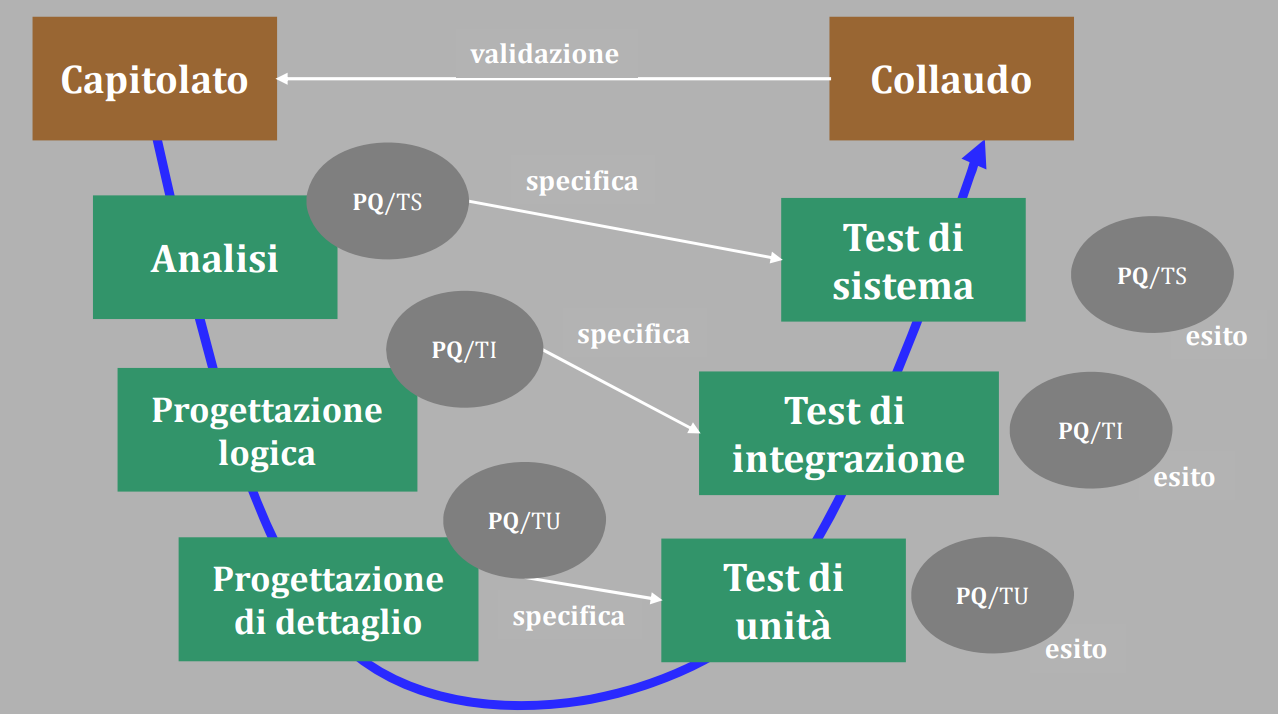
\includegraphics[width=\textwidth]{res/img/modelloV.png}
\end{figure}
Lo stato di integrazione di un prodotto software è rappresentabile in livelli, ognuno dei quali corrisponde ad una specifica revisione tecnica. Il modello a "V" rappresenta in maniera schematica la corrispondenza tra la tipologia di test e il livello del ciclo di vita software in cui essi vengono eseguiti. A ognuno di questi livelli, corrisponde una tipologia di test specifica. A partire dall'implementazione con i test di unità, si effettuano verifiche del prodotto sempre più complete sino ad arrivare al collaudo finale.

\subparagraph*{Test di unità}
Vengono effettuate delle prove sulle unità che compongono il prodotto software. Le unità rappresentano la più piccola parte del prodotto che è possibile eseguire e verificare autonomamente. Questa tipologia di test è effettuata con l'ausilio degli \textit{stub\glo} e dei \textit{driver\glos}.

\subparagraph*{Test di integrazione}
Test che agiscono a livello di componente. Possono essere eseguiti solo su un insieme di unità precedentemente testate. Il compito dei test di integrazione è di verificare se le unità presentano il comportamento atteso quando operano insieme a livello di componente.

\subparagraph*{Test di sistema}
Si basano sull'intero sistema e hanno lo scopo di verificare il funzionamento del prodotto dopo l'unione delle varie componenti che lo costituiscono. Essi dovranno verificare i requisiti definiti nell'\textit{Analisi dei requisiti 2.0.0\docs}.

\subparagraph*{Test di accettazione}
Verificano il prodotto nella sua completezza e si basano sull'esperienza del cliente rispetto ai bisogni espressi nel \textit{capitolato\glos}.

\subparagraph*{Test di regressione}
Vengono effettuati a seguito di una modifica apportata al sistema. Ogni modifica deve essere necessariamente seguita dall'esecuzione di tutti i test esistenti. Ciò servirà per accertare che la correttezza della modifica effettuata.


\subsubsection{Procedure}
\paragraph{Verifica della documentazione mediante inspection}
\begin{enumerate}
	\item ispezionare il documento o parte di esso seguendo i punti critici rilevati dalla tabella;
	\item notificare al responsabile della stesura del documento gli errori commessi;
	\item aggiornare la tabella degli errori comuni: se durante la verifica sono state rilevate delle ricorrenze per delle tipologie di errori non presenti all'interno della lista, dovranno essere riportate.
\end{enumerate}
\paragraph{Ottenimento e gestione esiti misurazioni}
\begin{enumerate}
	\item scegliere la metrica coinvolta per la misurazione della qualità di processo e di prodotto;
	\item calcolare il valore corrispondente all'avvenuta misurazione;
	\item verificare l'esito in base al risultato ottenuto;
	\item inserire i risultati ottenuti all'interno di un grafico che metta lo metta a paragone con quelli rilevati negli incrementi precedenti;
	\item inserire il grafico in appendice del PdQ.
\end{enumerate}

\subsubsection{Strumenti}
\paragraph{ESLint}
Strumento di analisi del codice utilizzato per lo sviluppo in JavaScript. Consente la creazione di codice leggibile e coerente con regole condivise dalla comunità degli sviluppatori. Esso è semplicemente installabile come \textit{plug-in\glo} di Visual Studio Code oppure mediante npm.

\paragraph{Mocha}
Framework per eseguire unit testing per applicazioni scritte in JavaScript, Typescript e per gli \textit{smart contract\glo} scritti in Solidity. Il framework è supportato da Visual Studio Code.

    \subsection{Validazione}
\subsubsection{Obiettivi}
La validazione del prodotto garantisce il prodotto sia conforme alle attese e, in particolare, a tutti i bisogni del cliente. Obiettivi del processo sono:
\begin{itemize}
	\item consentire il rilascio finale del prodotto sottostando i vincoli contrattuali concordati con il cliente;
	\item dimostrare la conformità del prodotto rispetto alle attese.
\end{itemize}

\subsubsection{Attività}
Fanno parte del processo di validazione i test di sistema e di accettazione (collaudo) descritti nel modello a V del capitolo precedente. Le attività comprendono il processo di validazione e che sono propedeutiche per quest'ultimo, sono le seguenti:
\begin{itemize}
	\item definizione chiara degli input e output del sistema;
	\item definizione dei valori accettabili dal sistema;
	\item definizione dell'ambiente (hardware e software) sul quale deve essere eseguito il prodotto;
	\item definizione degli errori che possono essere sollevati e di come essi vengono gestiti dal sistema;
	\item definizione della tipologia di validazione utilizzata e dei criteri di accettazione;
	\item riepilogo dei risultati ottenuti per l'accettazione del prodotto.
\end{itemize}

\subsubsection{Procedure}
\paragraph{Procedura di validazione del prodotto}
\begin{enumerate}
	\item identificazione degli elementi sui quali effettuare la validazione;
	\item pianificazione del metodo di validazione;
	\item ottenimento dei risultati per l'elemento validato;
	\item comparazione dei risultati ottenuti con quelli attesi e deduzione del grado di accettabilità.
\end{enumerate}
    \section{Processi Organizzativi}
	\subsection{Gestione}
		\subsubsection{Scopo}
  			%Questa parte del documento \`e necessaria per la creazione di un way of working ben organizzato permette di avere un flusso dei dati per definito dall'inizio alla fine
			Lo scopo di questo processo è quello di creare un way of working, utile ai membri del gruppo per organizzare e gestire i ruoli di ogni componente e le attività da svolgere.%CONTINUARE
  		\subsubsection{Aspettative}
  			Le aspettative per questo processo sono:
  			\begin{itemize}
  				\item definizione dei ruoli dei membri del gruppo;
  				\item pianificare le attività da seguire;
  				\item adoperare processi per regolare le attività e renderle economiche.
			\end{itemize}
   		\subsubsection{Descrizione}
   			Le attività che compongono questo processo sono:
   			\begin{itemize}
   				\item istanziazione dei processi;
   				\item assegnazione dei ruoli di progetto e dei compiti;
   				\item pianificazione e stima dei costi, tempi e risorse;
	   			\item esecuzione e controllo dei compiti;
   				\item verifica periodica dei compiti.
		   	\end{itemize}
   		\subsubsection{Ruoli di progetto}
   			Ciascun membro del gruppo, a rotazione, dovrà ricoprire il ruolo che gli viene affidato e che corrisponderà all'omonima figura aziendale. Nel \textit{Piano di Progetto 1.0.0} vengono organizzate e pianificate le attività assegnate a ciascun ruolo e ogni membro dovrà rispettare tali norme.

   			Nell'assegnamento dei ruoli si cercherà di evitare situazioni di conflitto, per garantire la qualità dei documenti e della verifica di quest'ultimi.

   			I ruoli sono descritti qui di seguito.
   			\paragraph{Analista} \mbox{}\\ \mbox{}\\
<<<<<<< HEAD
   				L'Analista è colui che effettua l'analisi dei problemi e del dominio applicativo. \`{E} una figura molto importante ai fini della riuscita del progetto, anche se non sarà sempre presente nello sviluppo di quest'ultimo. Se l'analista effettua degli errori nell'\textit{Analisi dei Requisiti 1.0.0}, questi possono portare a gravi problemi nella successiva progettazione del prodotto.
   				
=======
   				L'Analista è colui che effettua l'analisi dei problemi e del dominio applicativo. \`{E} figura molto importante ai fini della riuscita del progetto, anche se non sarà sempre presente nello sviluppo di quest'ultimo. Se l'analista effettua degli errori nell'\textit{Analisi dei Requisiti 1.0.0}, questi possono portare a gravi problemi nella successiva progettazione del prodotto.

>>>>>>> 1d58ec29b666ca4c2b9e6b789e3f96a0ac4367d9
   				I compiti principali dell'Analista sono:
   				\begin{itemize}
   					\item studiare e definire il problema da risolvere, e la sua complessità;
   					\item analizzare il dominio applicativo: utenti, ambiente d'uso;
   					%\item effettuare un'analisi dei bisogni descritti dal proponente e dal committente
   					\item produzione dello \textit{Studio di Fattibilità 1.0.0} e  dell'\textit{Analisi dei Requisiti 1.0.0}.
   				\end{itemize}
   			\paragraph{Progettista} \mbox{}\\ \mbox{}\\
   			Il Progettista è colui che si occupa degli aspetti tecnici e tecnologici del progetto. \`{E} inoltre responsabile delle scelte architetturali.

   			Partendo dall'analisi effettuata dall'\textit{Analista}, il suo compito è quello di trovare una soluzione ottimale ai problemi e ai requisiti individuati.

   			I suoi compiti principali sono:
   			\begin{itemize}
   				\item sviluppo dell'architettura secondo un insieme di best practice per garantire coerenza e consistenza;
   				\item effettuare scelte che portano ad una soluzione efficacie, efficiente e comprensibile rispetto ai requisiti, rientrando nei preventivi di costo e risorse;
   				\item rendere facilmente mantenibile il progetto;
   				\item sviluppo di un'architettura robusta , flessibile e sicura, che permetta al prodotto finale di rimanere funzionante e di effettuare modifiche a basso costo, in caso malfunzionamento;
   				\item applicazioni di soluzioni note e ottimizzate.
   			\end{itemize}
   			\paragraph{Programmatore} \mbox{}\\ \mbox{}\\
   			Il Programmatore è colui che si occupa della codifica del progetto e delle componenti di supporto, utili per effettuare le prove di verifica e validazione del prodotto.

   			Il suo compito principale è quello di realizzare l'architettura ideata dal \textit{Progettista}.

   			Tra i suoi compiti ci sono:
   			\begin{itemize}
   				\item implementare le decisioni del \textit{Progettista};
   				\item creazione e gestione delle componenti di supporto per verifica e validazione del codice.
   				\item stesura del \textit{Manuale Utente}.
   			\end{itemize}
   			\paragraph{Verificatore} \mbox{}\\ \mbox{}\\
   			Il Verificatore è colui che effettua il controllo sulle attività svolte, assicurandosi che esse siano conformi alle attese e alle norme stabilite.

   			I suoi compiti sono:
   			\begin{itemize}
   				\item verificare che le \textit{Norme di progetto 1.0.0} siano rispettate;
   				\item verificare la presenza di errori, e in caso segnalarli all'autore dell'oggetto preso in esame;
   				\item segnalare al \textit{Responsabile} eventuali situazioni di conflitto che violano ciò che è indicato nel \textit{Piano di Progetto 1.0.0}.
   			\end{itemize}
   			\paragraph{Responsabile} \mbox{}\\ \mbox{}\\
   			Il Responsabile è il punto di riferimento sia per il fornitore che per il committente. Inoltre è colui che raccoglie su di sè le responsabilità decisionali di scelta e approvazione e costituisce il centro di coordinamento per l'intero progetto.

   			I suoi compiti principali sono:
   			\begin{itemize}
   				\item approvazione della documentazione;
   				\item gestione, controllo e coordinamento delle risorse e dell'attività del gruppo;
   				\item studio e gestione dei rischi.
   			\end{itemize}
   			\paragraph{Amministratore} \mbox{}\\ \mbox{}\\
   			L'Amministratore è colui che controlla e amministra l'ambiente di lavoro.

   			L'Amministratore non deve operare scelte gestionale, ma aiutare il \textit{Responsabile} ad organizzare e gestire l'ambiente di lavoro.

   			I suoi compiti sono:
   			\begin{itemize}
   				\item gestione del versionamento e delle configurazioni del progetto;
   				\item risolvere problemi legati alla gestione dei processi;
   				\item amministrare le infrastrutture di supporto;
   				\item gestione della documentazione;
   				\item individuazione degli strumenti atti all'automazione dei processi;
   			\end{itemize}
   		\subsubsection{Procedure}
   			\paragraph{Gestione delle comunicazioni}
   				\subparagraph{Comunicazioni interne}
<<<<<<< HEAD
   					Per le comunicazione interne è stato deciso di utilizzare  Slack, un'applicazione di messaggistica multi piattaforma con funzionalità specifiche per gruppi di lavoro. Ogni canale è specifico per una determinata attività.
   				
   					All'interno di Slack sono stati aggiunti i seguenti canali:
=======
   					Per le comunicazione interne è stato deciso di utilizzare  Slack\glos, un'applicazione di messaggistica multi piattaforma con funzionalità specifiche per gruppi di lavoro. Ogni canale è specifico per una determinata attività.

   					All'interno di Slack\glo sono stati aggiunti i seguenti canali:
>>>>>>> 1d58ec29b666ca4c2b9e6b789e3f96a0ac4367d9
   					\begin{itemize}
   						\item \textbf{github}: per tutto ciò che riguarda github;
   						\item \textbf{pianificazione-incontri}: dove i membri del gruppo decidono quando effettuare i vari incontri.
   						\item \textbf{swe}: canale generale per discutere di ciò che riguarda l'organizzazione generale;
   						\item \textbf{logo}: per la scelta del logo del gruppo;

   					\end{itemize}
   					Altri canali telematici, sono stati aggiunti per gestire la stesura dei vari documenti quali:
   					\begin{itemize}
   						\item \textbf{norme\_di\_progetto}: per discutere e definire le Norme di Progetto alle quali attenersi durante le varie fasi di progetto;
   						\item \textbf{studio\_di\_fattibilità}: per redigere il relativo documento seguendo i criteri indicati;
   						\item \textbf{analisi\_requisiti}: per discutere e decidere i casi d'uso, i requisiti, i vincoli e tutto ciò che verrà inserito nel documento \textit{Analisi dei Requisiti 1.0.0};
   						\item \textbf{piano\_di\_progetto}: per decidere e discutere la ripartizione dei ruoli, le ore totali ad essi collegati nelle varie versioni del \textit{Piano di Progetto};
   						\item \textbf{piano\_di\_qualifica}: per decidere, discutere e fissare le strategie e gli obiettivi riguardanti la verifica, la validazione e la qualità.
   					\end{itemize}
   					Oltre all'applicazione Slack viene anche utilizzato un apposito gruppo Telegram e Google Hangouts, quando serve una comunicazione immediata, ma non è possibile trovarsi di persona.
   				\subparagraph{Comunicazioni esterne}
   					Le comunicazioni esterne sono affidate al \textit{Responsabile}, il quale si avvale dell'utilizzo della posta elettronica, attraverso l'indirizzo \href{mailto:tenners.unipd@gmail.com}{tenners.unipd@gmail.com}.
<<<<<<< HEAD
   					
   					Per comunicare con Red Babel, invece, si utilizza un canale Slack per la chat testuale e il servizio Google Hangouts per le chiamate.
   					
=======

   					Per comunicare con Red Babel, invece, si utilizza un canale Slack\glo per la chat testuale e il servizio Google Hangouts\glos o Skype\glo per le chiamate.

>>>>>>> 1d58ec29b666ca4c2b9e6b789e3f96a0ac4367d9
   					Il \textit{Responsabile} ha il compito di tenere informato i vari componenti del gruppo, in caso di loro assenza.
   			\paragraph{Gestione degli incontri}
   				\subparagraph{Incontri interni}
   					Le riunioni interne del gruppo sono organizzate dal \textit{Responsabile} in accordo con gli altri componenti del team, attraverso gli appositi canali.

   					Per ogni incontro viene esteso un \textit{Verbale}. Questo sarà redatto da un segretario, persona nominata dal responsabile, che dovrà tenere nota delle discussioni fatte e delle decisioni prese. La struttura dei verbali è descritta nel seguente paragrafo.
	   			\subparagraph{Incontri esterni}
   					Il \textit{Responsabile} ha il compito organizzare e comunicare gli incontri con il proponente o il committente. Se uno o più membri del gruppo, il proponente o il committente volessero organizzare un incontro, sarà compito del \textit{Responsabile} decidere una data, in accordo tra le parti, e successivamente di comunicarla tramite i canali appositi.

   					Come per gli incontri interni, anche per quelli esterni viene redatto un \textit{Verbale}.
   				\subparagraph{Verbali}
   					La prima parte contiene le informazioni generali quali:
   					\begin{itemize}
   						\item \textbf{Luogo}: indica il luogo dove è avvenuto l'incontro;
   						\item \textbf{Data}: indica la data dell'incontro, nel formato YYYY-MM-DD;
   						\item \textbf{Ora di inizio}: nel formato ventiquattro ore;
   						\item \textbf{Ora di fine}: nel formato ventiquattro ore;
   						\item \textbf{Partecipanti}: indica chi era presente alla riunione, sotto forma di elenco puntato;
   					\end{itemize}
   					La seconda parte contiene, sotto forma di elenco puntato, l'ordine del giorno con relativo resoconto per ogni punto.
<<<<<<< HEAD
   					
   					Ogni verbale interno verrà memorizzato con la seguente nomenclatura: verbaleInterno\_DATA.DD.
   					Mentre i verbali esterni verranno memorizzati come: verbaleEsterno\_DATA.DD.
   					
   					In entrambi i casi il formato della data sarà quello americano, mentre DD indica il numero di decisioni prese in quell'incontro.
   			\paragraph{Gestione degli strumenti di coordinamento}
   				\subparagraph{Tickecting}
   					Il tickecting permette ai vari membri del gruppo di monitorare, in qualsiasi momento, le attività in corso, permette al \textit{Responsabile} di monitorare l'andamento delle attività.
   					
   					Come strumento di tickecting e' stato deciso di usare i servizzi di project board offerti da GitHub.
   					
   					Su GitHub è stato creato un gruppo, il quale contiene varie reposity, in modo da separare le singole unità (esempio dividere il codice dai documenti).
   					La project board principale del gruppo è collegata  alle project board di ciascun reposity.
   					
   					Ogni project board è suddivisa in cinque sezioni:
   					\begin{itemize}
   						\item \textbf{To do}: indica le attività da svolgere;
   						\item \textbf{In progess}: indica tutte le attività che sono in fase di svolgimento;
   						\item \textbf{Review in progress}: indica le verifiche in fase di svolgimento;
   						\item \textbf{Review approved}: indica tutte le verifiche approvate;
=======

   					Ogni verbale interno verrà memorizzato con la seguente nomenclatura: VerbaleInterno DATA.
   					Mentre i verbali esterni verranno memorizzati come: VerbaleEsterno DATA.

   					In entrambi i casi il formato della data sarà quello americano, quindi anno-mese-giorno.
   			\paragraph{Gestione degli strumenti di coordinamento}
   				\subparagraph{Ticketing}
   					Il ticketing permette ai vari membri del gruppo di monitorare, in qualsiasi momento, le attività in corso, permette al \textit{Responsabile} di monitorare l'andamento delle attività.

   					Si è deciso di sfruttare i servizi di gestione issues e di projects boards offerti da GitHub\glos.
   					La projects boards è suddivisa in tre sezioni:
   					\begin{itemize}
   						\item \textbf{To do}: indica le attività da svolgere;
   						\item \textbf{In progress}: indica tutte le attività che sono in fase di svolgimento;
>>>>>>> 1d58ec29b666ca4c2b9e6b789e3f96a0ac4367d9
   						\item \textbf{Done}: indica tutte le attività completate;
   					\end{itemize}
   					Inoltre la project board del gruppo contiene i macro do to, i quali creano una milestone per il progetto.
   					
   					I to do vengono riportati in una milestone per il reposity di riferimento, e vengono analizzati e suddivisi in issues. Questo permette di inserire i vari requisiti usando un approccio top-down, e di usare un metodo botton-up per soddisfarli. 
   			\paragraph{Gestione rischi}\mbox{}\\ \mbox{}\\
   				Il \textit{Responsabile} ha il compito di individuare i rischi descritti nel \textit{Piano di Progetto}, e una volta trovati, inserirli nell'analisi dei rischi.

   				La procedura da seguire per la gestione dei rischi è la seguente:
   				\begin{itemize}
   					\item individuare problemi non calcolati e monitorare i rischi già previsti;
   					\item registrare ogni riscontro previsto dei rischi nel \textit{Piano di Progetto 1.0.0};
   					\item aggiungere i nuovi rischi individuati nel \textit{Piano di Progetto 1.0.0};
   					\item  se necessario, ridefinire le strategie di gestione dei rischi.
   				\end{itemize}
   		\subsubsection{Strumenti}
   			Il gruppo durante lo svolgimento del progetto ha utilizzato o utilizzerà i seguenti strumenti:
   			\begin{itemize}
   				\item \textbf{Telegram}: come strumento di messaggistica.
   				\item \textbf{Slack}: come strumento di comunicazione interna ed eventualmente con il proponente;
   				\item \textbf{Git}: come sistema di controllo di versionamento;
   				\item \textbf{Gitflow}: come interfaccia per usare, più comodamente, Git da Desktop;
   				\item \textbf{GitHub}: come strumento per il versionamento e il salvataggio in remoto di tutti i file legati al progetto;
   				\item \textbf{Hangouts}: come strumento per effettuare videoconferenze e chiamate VoIP;
   				\item \textbf{Sistemi Operativi}: i requisiti non prevedono di utilizzare un sistema operativo specifico, per questo verranno usati, dai membri del team, Windows, MacOS, sistemi di distribuzione Linux.
   			\end{itemize}
   		\subsubsection{Formazione}
<<<<<<< HEAD
   			Ogni singolo membro dovrà studiare in maniera autonoma le tecnologie da impiegare per la realizzazione del progetto. I membri del gruppo potranno creare delle guide, in modo del tutto informale relative ad un singolo argomento, per facilitare l'apprendimento ai restanti componenti del gruppo.
   			
   			Le guide utilizzate sono:
   			\begin{itemize}
   				\item GitHub: \href{https://github.com}{https://github.com};
   				\item \LaTeX: \href{https://www.latex-project.org/}{https://www.latex-project.org/};
   				\item  AWS: \href{https://docs.aws.amazon.com/}{https://docs.aws.amazon.com/};
   				\item Ethereum\glos: \href{https://ethereum.org/}{https://ethereum.org/};
   				\item Solidity: \href{https://solidity.readthedocs.io/en/develop/}{https://solidity.readthedocs.io/en/develop/};
   				\item Trulle suite: \href{https://www.trufflesuite.com/tutorials/ethereum-overview}{https://www.trufflesuite.com/tutorials/ethereum-overview};
   				\item Web3: \href{https://web3js.readthedocs.io/en/v1.2.4/}{https://web3js.readthedocs.io/en/v1.2.4/};
   				\item Node.js: \href{https://nodejs.org/it/docs/}{https://nodejs.org/it/docs/};
   				\item ESLint: \href{https://github.com/eslint/eslint}{https://github.com/eslint/eslint}.
   			\end{itemize}
=======
   			\paragraph{Formazione dei membri del gruppo}%\mbox{}\\ \mbox{}\\
   			\paragraph{Guide e materiale utilizzato}%\mbox{}\\ \mbox{}\\
>>>>>>> 1d58ec29b666ca4c2b9e6b789e3f96a0ac4367d9

    \appendix \section{Standard e modelli di riferimento}
\subsection{ISO/IEC 9126}
Lo standard ISO/IEC 9126 fornisce l'insieme delle caratteristiche rilevati che concorrono nel garantire la qualità di un prodotto. Esse sono suddivise in tre categorie:
\begin{itemize}
	\item \textbf{Qualità interne:} riguardanti le proprietà statiche e strutturali del software;
	\item \textbf{Qualità esterne:} riguardanti le proprietà dinamiche e comportamentali del prodotto;
	\item \textbf{Qualità d'uso:} relative alla percezione dell'utente finale.
\end{itemize}
Le tipologie di Qualità appena descritte sono fortemente influenzate l'una con l'altra. Le Qualità esterne ed interne descritte, sono ulteriormente specificate da altre sotto-caratteristiche, come verrà elencato in seguito:
\begin{itemize}
	\item \textbf{Funzionalità:} capacità di un prodotto software di fornire funzioni che soddisfino le esigenze stabilite. È caratterizzata da:
	\begin{itemize}
		\item \textbf{Appropriatezza:} capacità del prodotto di fornire un appropriato insieme di funzioni per i bisogni dell'utente;
		\item \textbf{Accuratezza:} capacità del prodotto di fornire i risultati attesi;
		\item \textbf{Interoperabilità:} capacità del prodotto di interagire con uno o più sistemi;
		\item \textbf{Conformità:} capacità del prodotto di aderire a degli standard consolidati;
		\item \textbf{Sicurezza:} capacità del prodotto di proteggere informazioni e dati sensibili.
	\end{itemize}
	\item \textbf{Affidabilità:} capacità del prodotto di mantenere un livello di prestazioni se soggetto a input differenti. È caratterizzata da:
	\begin{itemize}
		\item \textbf{Maturità:} capacità di un prodotto di evitare che si verificano errori o malfunzionamenti;
		\item \textbf{Tolleranza:} capacità di mantenere il livello prestativo anche in presenza di malfunzionamenti o usi scorretti del prodotto;
		\item \textbf{Interoperabilità:} capacità di un prodotto di ripristinare il livello appropriato di prestazioni in seguito a un malfunzionamento;
		\item \textbf{Recuperabilità:} capacità del prodotto di aderire a degli standard consolidati;
		\item \textbf{Aderenza:} capacità del prodotto di aderire a standard consolidati inerenti all'affidabilità.
	\end{itemize}
	\item \textbf{Usabilità:} capacità del prodotto software di essere compreso ed appreso dall'utente. È caratterizzata da:
	\begin{itemize}
		\item \textbf{Comprensibilità:} capacità del prodotto di essere utilizzata adeguatamente;
		\item \textbf{Apprendibilità:} esprime la velocità di apprendimento delle funzionalità del prodotto da parte di un utente;
		\item \textbf{Operabilità:} esprime l'indipendenza nell'utilizzo delle funzionalità data agli utenti;
		\item \textbf{Attrattivà:} esprime il grado di piacevolezza nell'utilizzo del prodotto;
		\item \textbf{Conformità:} capacità del prodotto di aderire a standard consolidati inerenti all'usabilità.
	\end{itemize}
	\item \textbf{Manutenibilità:} capacità del prodotto di essere posto sotto manutenzione e di essere modificato. È caratterizzata da:
	\begin{itemize}
		\item \textbf{Analizzabilità:} capacità che il prodotto ha di essere studiato e compreso per rilevare eventuali malfunzionamenti;
		\item \textbf{Modificabilità:} capacità del prodotto di essere modificato in seguito a malfunzionamenti senza la necessità di cambiare parti al di fuori di quella interessata dall'errore;
		\item \textbf{Stabilità:} capacità del software di evitare effetti inaspettati derivanti da modifiche errate;
		\item \textbf{Testabilità:} capacità del software di essere testato.
	\end{itemize}
	\item \textbf{Portabilità:} capacità del prodotto di non dipendere dal software, hardware o ambiente di esecuzione. È caratterizzata da:
	\begin{itemize}
		\item \textbf{Adattabilità:} capacità di cambiare ambiente di esecuzione senza dover apportare modifiche al prodotto;
		\item \textbf{Installabilità:} capacità di essere correttamente e facilmente installato indipendentemente dall'ambiente di utilizzo;
		\item \textbf{Conformità:} capacità del prodotto di aderire a standard consolidati inerenti alla portabilità;
		\item \textbf{Sostituibilità:} capacità del prodotto di compiere le stesse funzionalità di un sistema costruito per gli stessi scopi.
	\end{itemize}
\end{itemize}

\subsection{CMMI}
Il CMMI (Capability Maturity Model Integration) è un modello che fornisce le linee guida per migliorare stato di maturazione dei processi all'interno di un progetto software.
Questo modello descrive una strategia basata su 5 differenti livelli, ognuno dei quali ci fornisce delle informazioni sullo stato di maturazione del processo:
\begin{itemize}
	\item \textbf{Initial:} rappresenta il livello iniziale in cui i processi non hanno ancora regole e procedure stabilite e risultano non documentati adeguatamente;
	\item \textbf{Managed:} i processi principali sono organizzati, documentati e dunque anche ripetibili;
	\item \textbf{Defined:} i processi sono standardizzati e mantenuti efficaci ed aggiornati;
	\item \textbf{Quantitatively managed:} i processi, già ben organizzati e standardizzati, sono oggetto di processo di misurazione;
	\item \textbf{Optimizing:} i risultati ottenuti permettono il confronto e il miglioramento continuo. 
\end{itemize}

\end{document}
